\documentclass[utf8]{report}

\usepackage[utf8]{inputenc}

\usepackage{newtxtext}
\usepackage{newtxmath}

\usepackage[cm]{fullpage}
\setlength{\columnsep}{1cm}

\setlength{\parindent}{0pt}
\setlength{\parskip}{\smallskipamount}

\usepackage{tikz}
\usepackage{pgfplots}
\pgfplotsset{compat=1.5}
\usetikzlibrary{calc}

%\usepackage{fullpage}

\usepackage[colorlinks=true,destlabel=true]{hyperref}
\hypersetup{extension = }

\newcommand{\safety}[1]{%
\smallskip
\resizebox{\columnwidth}{!}{\fbox{\fbox{\begin{minipage}{0.96\linewidth}\emph{#1}\end{minipage}}}}%
\smallskip
}

\newcommand{\unit}[1]{\ensuremath{\mathrm{#1}}}
\newcommand{\micron}{\mbox{$\mu$m}}
\newcommand{\var}[1]{\ensuremath{\left<\mathrm{#1}\right>}}

\newenvironment{labeled}[1]{%
  \begin{tikzpicture}[
    label/.style={
      minimum height=0.8cm,
      red,
      thick,
      <-,
      rectangle,
      draw=red
    }
  ]
  \node at (0,0) {#1};
}{
  \end{tikzpicture}
}
\newcommand{\arrowandlabel}[4]{
  \draw[label] #1 -- #2 node [label,anchor=#3] {#4};
}
\newcommand{\arrowonly}[2]{
  \draw[label] #1 -- #2;
}
\newcommand{\dummylabel}[2]{
  \draw[label,white] #1 node [label,anchor=#2,draw=white] {};
}

% https://tex.stackexchange.com/questions/52317/pdftex-warning-version-allowed
\pdfminorversion=7

\newif\ifcoatli
\coatlifalse
\newif\ifcolibri
\colibrifalse
\newif\ifddoti
\ddotifalse



\coatlitrue

\newcommand{\projectname}{COATLI}
\newcommand{\projectexternalipname}{coatli.astrossp.unam.mx}
\newcommand{\projectexternalipaddress}{132.248.4.23}
\newcommand{\projectinterfaceurl}{http://\projectexternalipname/}
\newcommand{\projectaccount}{coatli}
\newcommand{\windlimit}{20}

\newcommand{\diego}[1]{{\color{blue}{Diego: \textbf\small{#1}}}}
\newcommand{\magui}[1]{{\color{red}{Magui: \textbf\small{#1}}}}
\newcommand{\rosa}[1]{{\color{green}{Rosa: \textbf\small{#1}}}}

\newcommand{\Is}{\mbox{$I_\mathrm{s}$}}

%\includeonly{chapter-operations}

\begin{document}

%!TEX root = technical-manual.tex

\pagestyle{empty}

\begin{centering}

\ifcoatlioan
\bigskip
\bigskip
\includegraphics[width=\linewidth]{figures/logo-gn.png}
\bigskip
\bigskip
{
 \Large
 \bfseries 
 COATLI/OAN Technical Manual
 \par
}
\bigskip
{
\baselineskip=10pt
 \large
 Fernando~Ángeles,
 Rosa~L.~Becerra,
 Oscar~Chapa,\\
 Salvador~Cuevas~Cardona,
 Alejandro~S.~Farah,
 Jorge~Fuentes-Fernández\\
 Rosalía~Langarica~Lebre,
 Fernando~Quirós,
 Carlos~G.~Román-Zúñiga\\
 Carlos~G.~Tejada
 and
 Alan~M.~Watson
 \par
}
\bigskip
{
 \large
 \itshape 
 Instituto de Astronomía\\
 Universidad Nacional Autónoma de México
 \par
}
\bigskip
{
 \large
 4 June 2022
}
\fi

\ifddotioan
\bigskip
\bigskip

{
 \Large
 \bfseries 
 DDOTI/OAN Technical Manual
 \par
}
\bigskip
\bigskip
\includegraphics[width=\linewidth]{figures/frontmatter-ddotioan.jpg}

\bigskip
\bigskip
{
\baselineskip=10pt
 \large
 Fernando~Ángeles,
 Rosa~L.~Becerra-Godínez,
 Alejandro~S.~Farah,
 William~H.~Lee,
 Fernando~Quirós,
 Carlos~G.~Román-Zúñiga,
 Carlos~G.~Tejada,
 and
 Alan~M.~Watson
 \par
}
\bigskip
{
 \large
 \itshape 
 Instituto de Astronomía\\
 Universidad Nacional Autónoma de México
 \par
}
\bigskip
{
 \large
 4 June 2022
}
\fi

\end{centering}

\newpage

\pagestyle{plain}

%\twocolumn

\tableofcontents



\twocolumn

\chapter{Introduction}
\label{chapter:introduction}

\ifcolibri

This is the technical manual for the {\projectname} telescope control system (TCS). It has two aims. The first is to allow the COLIBRI staff to operate the telescope conventionally, issuing commands explicitly. The second is to allow the COLIBRI staff to manage the observing blocks for robotic operations.

\else

This is the technical manual for the {\projectname} installation, telescope, and instrument. It has two aims. The first is to provide clear instructions to the OAN/SPM technical staff supporting routine operations. The second is to aid {\projectname} and OAN/SPM technical staff perform preventative and corrective maintenance of the equipment.

For an overview of the {\projectname} project, we recommend our 2016 SPIE paper:

\ifcoatli
\begin{itemize}
\item “\href{bibliography/spie-coatli-2016.pdf}{COATLI: an all-sky robotic optical imager with 0.3 arcsec image quality}”,   Watson et al.\ 2016, Proc.\ SPIE, 9908, 99085O-2
\end{itemize}
\fi

\ifddoti
\begin{itemize}
\item “\href{bibliography/spie-ddoti-2016.pdf}{DDOTI: the deca-degree optical transient imager}”, Watson et al.\ 2016, Proc.\ SPIE, 9910, 99100G
\end{itemize}
\fi

\ifcoatli
{\projectname} has been funded by CONACyT (LN 232649, 260369, and 271117)
and the Universidad Nacional Aut\'onoma de M\'exico (CIC and
DGAPA/PAPIIT IT102715, IG100414, IN109408, and IN109418) and is operated and
maintained by the Observatorio Astron\'omico Nacional and the Instituto
de Astronom{\'\i}a of the Universidad Nacional Aut\'onoma de M\'exico.
\fi

\ifddoti
DDOTI is funded by CONACyT (LN 232649, LN 260369, LN 271117, and 277901), the Universidad Nacional Autónoma de México (CIC and DGAPA/PAPIIT IG100414, IT102715, AG100317, IN109418, IG100820, and IN105921), the NASA Goddard Space Flight Center, and the University of Maryland (NNX17AK54G). DDOTI is operated and maintained by the Observatorio Astronómico Nacional and the Instituto de Astronomía of the Universidad Nacional Autónoma de México. We acknowledge the contribution of Neil Gehrels to the development of DDOTI.
\fi

\fi

\include{part-operations}

\chapter{Safety}
\label{chapter:safety}


In this manual, safety instructions and observations are highlighted by boxes.
\section{Feedback}

If you encounter a dangerous situation that is specific to {\projectname} and is not covered by the rules below or if you have comments or suggestions on the existing rules, please inform the leaders of {\projectname}
\ifcoatli
(Alan Watson and Salvador Cuevas)
\fi
\ifddoti 
(Alan Watson and William Lee) 
\fi
and the Secretario Técnico of the OAN.

\section{Priorities}

\safety{
The safety priorities at {\projectname}, from highest to lowest, are:
\begin{enumerate}
\item Avoiding injury and death to personnel.
\item Avoiding damage or loss of equipment.
\item Observing and data preservation.
\end{enumerate}
}

\section{Personnel Safety}
\label{section:personnel-safety}

The {\projectname} installation is potentially one of the most dangerous installations at the OAN/SPM. Personnel safety is more important than equipment safety or observations. The following  rules are designed to maintain personnel safety and must be followed at all times.

%\safety{You must not work alone on the open platform or on the balconies.} 

\safety{When you work on the balconies or the structure of the tower, you must be accompanied by at least one other person.}

\safety{When you work on the platform, you must either (a) be accompanied by at least one other person or (b) be in contact by radio or chat with another person on the mountain and advise them before and after each ascent or descent.}

\safety{When working on the platform, close it partially or fully if possible.}

You should have someone to close the enclosure manually after you have entered and open it manually for you to leave. Remember that you must have a radio on hand.

\safety{You must use a safety harness, line, and helmet whenever you are on the  platform or balconies or to ascend the tower. When you are working on the balcony or another position from which you might fall, attach your line to one of the eyes, to the balcony rail, or to something equivalently strong. In cold weather, we strongly recommend using gloves.} 

The main platform is about 5 meters above the walkways. A fall from this height can easily kill.

Safety harnesses, lines, and helmets are stored in the shed.

The line can be attached to various points: the eyes in the platform floor and balconies installed specifically for this purpose, the balcony safety rails, and other parts of the platform or tower structure.

The helmet will protect you from collisions with the telescopes, if you fall, and from falling objects.

\safety{You must use a safety helmet if you are working under the platform or balconies.}

The main platform is about 5 meters above the walkways. An impact from an object falling from this height can easily kill.

Safety helmets are stored on the shed.

\safety{Transport equipment and tools to and from the platform using the appropriate equipment provided: ropes, locking carabiners, locking hooks, straps, a tool carrier, and an equipment bag.}

This equipment, shown in Figure~\ref{figure:safety-transport}, is stored in the project cabinet in the ground-floor of the 84-cm telescope. Using this equipment in an appropriate manner will significantly reduce the risk of something falling. When you use the rope, you can fasten the upper end to one of the eyes in the platform using a locking carabiners. When lifting heavy equipment to the platform, consider using the locking hook.

\begin{figure}
\begin{center}
\resizebox{\linewidth}{!}{
\includegraphics[width=0.50\linewidth]{figures/safety-rope}
\includegraphics[width=0.50\linewidth]{figures/safety-straps.jpg}
}
\resizebox{\linewidth}{!}{
\includegraphics[width=0.50\linewidth]{figures/safety-tools.jpg}
\includegraphics[width=0.50\linewidth]{figures/safety-bag.jpg}
}
\end{center}
\caption{Equipment to safely transport equipment to and from the platform: ropes, locking carabiners, straps, a tool carrier, and an equipment bag.}
\label{figure:safety-transport}
\end{figure}

\safety{Return equipment and tools to their usual storage location when you have finished using them.}

This ensures that equipment can be found when it is next needed. This is especially important for safety equipment.

\safety{If you wish to ascend to the platform or balconies, you must put the enclosure in local mode.}

In remote mode the enclosure can close without warning.

\safety{You may only be on the platform or balconies if it is strictly necessary.}

The platform and balconies are not a vantage points. You must only be on them to work on equipment.

\safety{You may only be on the platform or balconies at night if you need to close the enclosure manually or are commissioning, testing, or tuning equipment on the sky.}

If there is a failure at night, you must not ascend to the platform to fix it. Instead, you must abandon the night’s observations and attempt to close the enclosure from the shed. You may only ascend to the platform at night if you need to close the enclosure manually.

\safety{You may only be on the platform or balconies in poor conditions if you need to close the enclosure manually.}

Poor conditions include high wind, snow, and rain. 

You must not perform maintenance in poor conditions.

You may only climb the platform in poor conditions if you need to close the enclosure manually.

\safety{Do not walk on the elevated areas at the ends of the platform.}

These areas are not load-bearing. If you walk on them, it is likely that they will collapse and you will fall.

\safety{If you need to summon help and do not have a portable radio, you can use chat over WiFi or the static emergency radio located between the 84-cm building and DDOTI.} 

\safety{You must physically disconnect mains power before working on an electronics box.}

Note that the platform box has two mains connectors, one for regulated power and one for unregulated power. The other boxes have only one mains connector, for regulated power.

Using the switch is not enough; it is present to allow the equipment to be rebooted. Besides, the unregulated power to the platform box is not switched.

\safety{Be extremely careful when working inside the enclosure, covers, and secondary cabinets as they use 220 VAC.}


\section{Equipment Safety}

\safety{Only open the enclosure explicitly when conditions are benign.
Conditions are not benign if:
\begin{enumerate}
\item It is raining or snowing.
\item The humidity is 85\% or higher and rising or previously reached 90\% and has not yet fallen below 80\%.
\item The wind average speed has been {\windlimit} km/h or greater at any moment in the previous 30 minutes.  
\item There are other circumstance which, in the judgment of observatory technical staff, dictate that it is not safe to open. These include but are not limited to smoke or ash from forest fires and snow blowing off the nearby trees.
\end{enumerate}
}

Rules 1 to 3 are implemented in the {\projectname} weather server. If you check the {\projectname} web interface (see \S\ref{chapter:interface}), there is a summary line for the weather that says “may be open”, conditions are benign and you may open with the permission of the observatory staff. If it does not, conditions are not benign and you must not open.

Note that the rules for opening the other telescopes specify a wind limit of 45 km/h. The limit for {\projectname} is currently lower until we have greater confidence in its reliability and performance in high winds.

\safety{Before opening the enclosure, check on the webcams in the interface (see \S\ref{chapter:interface}) that the telescope is not pointed to towards the sun.}

\ifcoatli
In the home position, the telescope is pointed to the north pole with the telescope above the mount.
\fi
\ifddoti
In the home position, the telescope is pointed to the north pole with the telescopes to the east and west of the mount.
\fi


\safety{The enclosure controller (see \S\ref{chapter:enclosure}) should normally be switched on at all times in order to keep the electromagnetic lock activated.}

If the lock is not activated, the wind can open the roof a few centimeters and allow the ingress of rain or snow.

\safety{In case of fire, there is an extinguisher in the shed.}

If you do fight a fire, remember that personnel safety is more important than equipment safety.


\chapter{Documentation}
\label{chapter:documentation}

This chapter describes the documentation of {\projectname}.

\section{Access}

The address of the {\projectname} mountain-top web site is:
\begin{quotation}
\url{\projectinterfaceurl}
\end{quotation}

The web site contains the interface and documentation.

The documentation is available directly to computers on the mountain-top network and the Instituto de Astronomía networks in Ensenada and CU.

\section{Local Access}
\label{section:interface-access-mac}

The documentation can be accessed locally by OAN technical staff using the Mac in the shed.

If you need to log into the Mac, use the “{\projectaccount}” account with password “{\projectaccount}”. After this, open Safari and follow the instructions above for access to the web site.


\include{chapter-interface}
\chapter{Operations}
\label{chapter:operations}

{\projectname} is in regular robotic operation under the responsibility of the observatory staff. Weather permitting, {\projectname} will operate from 30 minutes before sunset to the end of morning astronomical twilight.

\section{Participants}

By “observatory staff” we refer to the telescope operators, resident astronomers, and maintenance technicians. The actually division of responsibilities will be decided by the Secretario Técnico of the observatory.

By “team members” we refer to members of the {\projectname} technical teams.

\section{Communications}

Communication between the observatory staff and the team will take place primarily through the COATLI/DDOTI Workspace in Google Chat.

\section{Daily Operations}

The daily operating procedure is:

\begin{enumerate}

\item At the latest one hour before sunset, the observatory staff will carry out a review of the {\projectname} installation. 

This revision has three elements. The observatory staff will:

\begin{enumerate}
\item
Check that all of the control system servers are not showing errors in the web interface (see \S\ref{figure:interface-main-page}). If there are problems, attempt to solve them by pressing the “Restart” button in the web interface and giving the system a couple of minutes to restart. If that doesn't work, seek the help of a team member.
\item
Check that the webcams in the web interface are not showing an unusual situation.
\item
If necessary, carry out an on-site inspection of {\projectname}. For example, after a snowfall, it might not be obvious from the webcams whether snow remains on the roof of the enclosure.
\end{enumerate}

If the observatory staff consider that decisions to open and close the installation can be safely taken by the control system, they will enable the supervisor by pressing the “Enable” button in web interface (see \S\ref{figure:interface-main-page}). 

If the observatory staff considers that decisions to open and close the installation cannot be safely taken by the control system, they should explicitly force the supervisor to maintain the telescope closed by pressing the “Close” button in  the web interface (see \S\ref{figure:interface-main-page}).. 

The observatory staff will report the result of their inspection in the Google chat and will indicate whether they are enabling the supervisor or forcing it to close.

\item
If the supervisor is enabled and weather conditions are benign, the control system will:
\begin{enumerate}
\item
Open partially to cool about half an hour before sunset;
\item
Open completely to observe at sunset; and
\item
Close at the end of morning astronomical twilight.
\end{enumerate}

If the supervisor is enabled and weather conditions are not benign, the control system will not open (if closed) or will close (if open).

If the supervisor is enabled and weather conditions change from not benign to benign, the control system will open partially to cool (between half and hour before sunset and sunset) or open completely to observe (between sunset and the end of morning astronomical twilight).

\item
The supervisor considers weather conditions to be \emph{not benign} if:
\begin{enumerate}
\item It is raining or snowing.
\item The humidity is 85\% or higher and rising or previously reached 90\% and has not yet fallen below 80\%.
\item The wind average speed has been 30 km/h or greater at any moment in the previous 30 minutes.  
\end{enumerate}
Note that the rules for opening the other telescopes specify a wind limit of 45 km/h. The limit for {\projectname} is currently lower until we have greater confidence in its reliability and performance in high winds.

\item
The observatory staff will monitor {\projectname} during the night. Their primary responsibilities are:
\begin{enumerate}
\item If the observatory staff consider that decisions to open and close the installation can be safely taken by the control system, they should enable the supervisor by pressing the “Enable” button in the web interface (see \S\ref{figure:interface-main-page}) and report this in the Google chat.
\item If the observatory staff consider that decisions to open and close the installation cannot be safely taken by the control system, they must explicitly force the supervisor to maintain the telescope closed by pressing the “Close” button in the web interface (see \S\ref{figure:interface-main-page}) and report this in the Google chat. 
\item
The observatory staff should verify that the control system opens and closes as expected according to the weather conditions and the state of the supervisor. If it does not close, they should intervene as described in \S\ref{section:operations:interventions}.

\item
When the control system closes (at the end of the night, in response to weather conditions, or if the supervisor is forced to close), it switches the lights on for safety. At the end of the process, if the control system can determine that the enclosure closed correctly, it will switch the lights off. If it cannot, it will leave the lights switched on. Thus, if the lights are left on, this indicates that there was a problem during closing and the observatory staff should intervene as described in \S\ref{section:operations:interventions}.

\item
The observatory staff should report explicit changes to the supervisor state (e.g., use of the “Enable” and “Close” buttons) and any other relevant information in the Google chat.
\end{enumerate}

As their other duties permit, the observatory staff are encouraged to report other conditions or occurrences that might degrade the ability of the telescope to observe (e.g., failures of the control system or failures to focus) in the Google chat.

\item
During the evening and night, interventions by the observatory staff are limited to whatever is necessary to close {\projectname} and return it to a safe state. Once the observatory staff have intervened, {\projectname} must be closed and may not open again until the next day.

\item
Requests by team members for interventions beyond those needed to close {\projectname} correctly will be directed to the Secretario Técnico of the observatory.
\end{enumerate}

\section{Interventions to Close}
\label{section:operations:interventions}

The control system should normally operate without problems and with minimal action on the part of the observatory staff beyond setting the supervisor mode. However, in the event of a failure, the observatory staff may need to intervene to close.

If the control system does not close when expected or does not close correctly, the observatory staff should:

\begin{enumerate}
\item
First attempt to close normally:
\begin{enumerate}
\item
Press the “Close” button in web interface (see \S\ref{figure:interface-main-page}). This should turn on the enclosure lights and close.
\item
Check the web interface and webcams for success or failure.
\end{enumerate}
\item
If that fails, attempt an emergency close:
\begin{enumerate}
\item
Press the “Emergency Close” button in the web interface (see \S\ref{interface-close-button}). This should turn on the enclosure lights and close.
\item
Check the web interface and webcams for success or failure.
\end{enumerate}
\item
If that fails, close the enclosure locally according to the procedure in \S\ref{section:enclosure-opening-or-closing-in-local-mode}.
\item
If that fails, close the enclosure manually according to the procedures in 
\S\ref{section:enclosure-manual-opening-or-closing-without-power}.
\end{enumerate}

\section{Weekly Inspection}

The observatory staff should carry out a physical inspection of the installations during daytime at least once per week (if weather conditions permit). The Secretario Técnico will determine the schedule for this inspection.

\subsubsection{Safety Considerations}

\safety{You must use a safety harness, line, and helmet whenever you are on the  platform or balconies or to ascend the tower. Attach your line to one of the fasteners, to the balcony rail, or to something equivalently strong.}

\safety{You must use a safety helmet if you are working under the platform or balconies.}

\safety{See \S\ref{section:personnel-safety} for a more complete discussion of safety.}

\subsubsection{Requirements}

You will need:
\begin{itemize}
\item At least two persons.
\item The key to the shed (see \S\ref{section:shed}).
\item Weather conditions adequate for opening the enclosure and ascending to the platform.
\end{itemize}

\subsubsection{Procedure}

\begin{enumerate}
\item
Verify that there is a fire extinguisher in the shed.
\item 
Verify that the web interface open on the Raspberry Pi in the shed. If it is not, open it by following the procedures in \S\ref{section:interface-local-access}.
\item 
Inspect the inside of the shed. 
\item 
Inspect the columns and underside of the platform.
\item
Open the enclosure locally to 60 degrees using the procedure in \S\ref{section:enclosure-opening-or-closing-in-local-mode}.
\item
One person should ascend to the platform to inspect: the electronics boxes, the instrument, the telescope, the mount, and the platform.
\item
Close the enclosure locally using the procedure in \S\ref{section:enclosure-opening-or-closing-in-local-mode}, but leave the enclosure controller in local mode.
\item
The person on the platform should inspect the enclosure roof from the inside.
\item
Open the enclosure locally using the procedure in \S\ref{section:enclosure-opening-or-closing-in-local-mode}.
\item
The person on the platform should descend.
\item
Leave the enclosure controller in remote mode.
\item
Report that the revision has been carried out and any anomalies in COATLI/DDOTI Workspace in Google Chat.
\end{enumerate}

\section{Soft Shut-Down and Start-Up}

A “soft” shut-down is appropriate for circumstances in which electrical power will continue to be supplied to {\projectname}. This is the normal situation over the winter break. In this case, we can leave the computers on and rely on the electromagnet to maintain the enclosure closed.

\subsection{Soft Shut-Down}
\label{section:soft-shut-down}

\subsubsection{Safety Considerations}

\safety{You must use a safety harness, line, and helmet whenever you are on the  platform or balconies or to ascend the tower. Attach your line to one of the fasteners, to the balcony rail, or to something equivalently strong.} 

\safety{You must use a safety helmet if you are working under the platform or balconies.}

\safety{The enclosure controller cabinet uses 220 VAC. Switch off the power using the main power switch on the door before working inside the cabinet (see Figure \S\ref{figure:enclosure-controller-door}) .}

\safety{See \S\ref{section:personnel-safety} for a more complete discussion of safety.}

\subsubsection{Requirements}

You will need:
\begin{itemize}
\item At least two persons.
\item The key to the shed (see \S\ref{section:shed}).
\item Weather conditions adequate for opening the enclosure and ascending to the platform.
\ifddoti
\item A clean tarpaulin, one long rope,  and one short red cord
\fi
\ifcoatli
\item A clean tarpaulin and one short red cord.
\fi
You can find clean tarpaulins in the shelves next to the cabinet in the 84-cm and rope in the tool-drawer of the cabinet.
\end{itemize}

\subsubsection{Procedure}

\begin{enumerate}

\item
Place the enclosure in local mode.

Move the enclosure controller mode selector switch to “LOCAL” (see Figure \S\ref{figure:enclosure-controller-door}).
\item
If the weather permits, open the enclosure to 60 deg.

Set the angle selector switch to 60 deg and then press and hold the open button until the green light goes out.

\item
Both persons should ascend to the platform.

\item
\ifcoatli
Verify that the telescope is in the parked position, pointed at the north pole and with the telescope above the mount. If not, release the break on the mount by pressing the “BRAKE” button and move it to this position. See Figure~\ref{figure:tarpaulin-before}.
\fi
\ifddoti
Move the telescope so that it is pointed vertically with the CCDs on the bottom and the focusers on the top. To move the telescope, release the brake on the mount by pressing the “BRAKE” button. See Figure~ref{figure:tarpaulin-before}.
\fi

\begin{figure}
\ifcoatli
\begin{center}
\includegraphics[width=0.8\linewidth]{figures/tarpaulin-coatli-before.jpg}
\end{center}
\caption{The telescope prior to being covered by a tarpaulin, pointed at the north pole and with the telescope above the mount. }
\fi
\ifddoti
\begin{center}
\includegraphics[width=0.8\linewidth]{figures/tarpaulin-ddoti-before.jpg}
\end{center}
\caption{The telescope prior to being covered by a tarpaulin, pointed vertically with the CCDs on the bottom and the focusers on the top. }
\fi
\label{figure:tarpaulin-before}
\end{figure}

\item
Press the mount emergency stop button.

\begin{figure*}
\ifcoatli
\begin{center}
\includegraphics[width=0.65\linewidth]{figures/tarpaulin-coatli.jpg}
\end{center}
\caption{The telescope covered by a tarpaulin.}
\fi
\ifddoti
\begin{center}
\includegraphics[width=0.45\linewidth]{figures/tarpaulin-ddoti.jpg}
\includegraphics[width=0.45\linewidth]{figures/tarpaulin-ddoti-annotated.jpg}
\end{center}
\caption{The telescope covered by a tarpaulin. The rope should go around the telescopes (green lines on the right, solid in front and dashed behind), below the two electronics boxes but \emph{above the lower end of the telescopes and the CCDs}, and then over the the telescopes (red lines on the right), between the east and west sets, and fasten on itself to prevent it slipping down. The loose ends of the tarpaulin should be gathered and tied with a short red rope.  The tarpaulin and the ropes \emph{must not come into contact with the CCDs} and must not place any stress on them.}
\fi
\label{figure:tarpaulin}
\end{figure*}

\item
Cover the telescope with a tarpaulin.
\ifcoatli
Gather the loose ends of the tarpaulin below and fasten them with a short red cord. See Figure~\ref{figure:tarpaulin}.
\fi
\ifddoti
Be very careful not to place stress on the CCDs.

Wrap the long rope around the telescopes and tarpaulin, below the two electronics boxes but above the lower end of the telescopes and the CCDs, and then pass a loop over the telescopes, between the east and west sets, and fasten the rope on itself to prevent it slipping down. Gather the loose ends of the tarpaulin below and fasten them with a short red cord. See Figure~\ref{figure:tarpaulin}.

{\itshape\bfseries We repeat: The tarpaulin and the ropes must not come into contact with the CCDs and must not place any stress on them. The tarpaulin and ropes can only come into contact with the telescope tubes, focusers, and electronics boxes.}

\fi

\item
Descend from the platform.

\item 
Close the enclosure.

Press and hold the close button until the green light goes out.

\item
Switch off the enclosure controller.

Move the main power switch on the controller door from ON to OFF. (see Figure \S\ref{figure:enclosure-controller-door}).
\item
Open the enclosure controller cabinet.

\item
Engage the manual lock. This switches on the enclosure electromagnet and actuates the enclosure emergency stop buttons. This ensures that the electromagnet stays energized even if the PLC fails and that the PLC cannot attempt to open the enclosure.

Move the manual lock switch inside the enclosure controller cabinet from OFF to ON. See Figure~\ref{figure:enclosure-controller-manual-lock-switch}.

\item
Close the enclosure controller cabinet.

\item
Switch on the enclosure controller.

Move the main power switch on the controller door from OFF to ON.

\item
Place the enclosure in remote mode.

Move the enclosure controller mode selector switch to “REMOTE”.

\item
\ifcoatli
Make sure the “PROHIBIDO EL PASO” sign is left in position at the bottom of the access stairs.
\fi
\ifddoti
Make sure the “PROHIBIDO EL PASO” signs are left in position at the bottom of the access ladders.
\fi

\item
Leave the shed locked. Return the shed keys to the tool box (see \S\ref{section:shed}).

\end{enumerate}

\subsection{Soft Start-Up}
\label{section:soft-start-up}

\subsubsection{Safety Considerations}

\safety{You must use a safety harness, line, and helmet whenever you are on the  platform or balconies or to ascend the tower. Attach your line to one of the fasteners, to the balcony rail, or to something equivalently strong.} 

\safety{You must use a safety helmet if you are working under the platform or balconies.}

\safety{The enclosure controller cabinet uses 220 VAC. Switch off the power using the switch on the door before working inside the cabinet.}

\safety{See \S\ref{section:personnel-safety} for a more complete discussion of safety.}

\subsubsection{Requirements}

You will need:
\begin{itemize}
\item At least two persons.
\item The key to the shed (see \S\ref{section:shed}).
\item Weather conditions adequate for opening the enclosure and ascending to the platform.
\end{itemize}

\subsubsection{Procedure}

\begin{enumerate}

\item
In the shed, switch off the enclosure controller.

Move the main power switch on the controller door from ON to OFF (see Figure \S\ref{figure:enclosure-controller-door}).

\item
Open the enclosure controller.

\item
Disengage the manual lock.

Move the manual lock switch inside the enclosure controller from ON to OFF. See Figure~\ref{figure:enclosure-controller-manual-lock-switch}.

\item
Close the enclosure controller.

\item
Switch on the enclosure controller.

Move the main power switch on the controller door from OFF to ON.

\item
Place the enclosure in local mode.

Move the enclosure controller mode selector switch to “LOCAL”.

\item
If the weather permits, open the enclosure to 60 deg.

Set the angle selector switch to 60 deg and then press and hold the open button until the green light goes out.

\item
Both persons should ascend to the platform.

\item
Remove the tarpaulin from the telescope.

\item Disengage the mount emergency stop button on the platform.

\item
\ifcoatli
Verify that the telescope is in the parked position, pointed at the northern horizon with the telescope on the west side of the pillar. If not, release the break on the mount by pressing the “BRAKE” button and move it to this position.
\fi
\ifddoti
Move the telescope to the parked position, pointed just below the northern horizon. To move the telescope, release the brake on the mount by pressing the “BRAKE” button.
\fi

\item Descent from the platform.

\item Close the enclosure. 

Press and hold the close button until the green light goes out.

\item
Place the enclosure in remote mode.

Move the enclosure controller mode selector switch to “REMOTE”.

\item
\ifcoatli
Make sure the “PROHIBIDO EL PASO” sign is left in position at the bottom of the access stairs.
\fi
\ifddoti
Make sure the “PROHIBIDO EL PASO” signs are left in position at the bottom of the access ladders.
\fi

\item
Leave the shed locked. Return the shed keys to the tool box (see \S\ref{section:shed}).

\item
Store the tarpaulin in the shelves next to the cabinet in the 84-cm and the rope in the tool-drawer of the cabinet.

\end{enumerate}

\section{Hard Shut-Down and Start-Up}

A “hard” shut-down is appropriate for circumstances in which electrical power will not continue to be supplied to {\projectname}. This has occurred, for example, in the evacuations for COVID-19 and when the observatory has been evacuated because of approaching storms. In this case, we must shut down the computers and cannot rely on the electromagnet to maintain the enclosure closed.

\subsection{Hard Shut-Down}

\subsubsection{Requirements}

You will need:

\begin{itemize}
    \item Two people plus the participation of a remote team member.
    \item The key to the shed (see \S\ref{section:shed-key}).
    \item Weather conditions adequate for opening the enclosure and ascending to the platform.
    \item The tarpaulin and ropes required for the soft shut-down (see \S\ref{section:soft-shut-down}).
    \item The two riveted plates, a riveter, and rivets.
\end{itemize}

\subsubsection{Procedure}

\begin{enumerate}
\item Perform a soft shut-down (see \S\ref{section:soft-shut-down}).
\item Communicate with the remote team member. They will:
\begin{enumerate}

    \item Halt the local access computer:

\begin{quote}\footnotesize
\ifcoatli
\begin{verbatim}
$ ssh coatli@coatli-console
console$ sudo halt
\end{verbatim}
\fi
\ifddoti
\begin{verbatim}
$ ssh ddoti@ddoti-console
console$ sudo halt
\end{verbatim}
\fi
\end{quote}
    
    \item Halt the TCS computers:

\begin{quote}\footnotesize
\ifcoatli
\begin{verbatim}
$ ssh coatli@coatli-control
control$ tcs haltsoon
\end{verbatim}
\fi
\ifddoti
\begin{verbatim}
$ ssh ddoti@ddoti-control
control$ tcs haltsoon
\end{verbatim}
\fi
\end{quote}

\end{enumerate}

\item Switch off the two UPSes, the 127 V UPS and the 220 V UPS.

On both UPSes, press the power button on the front panel for three seconds. The UPS will start to beep and will then switch off.

\item Switch off the power supply to the two UPSes.

Open the breaker panel on the wall next to the door. Switch off circuits A and B.

\item
Install the two riveted two plates, one on each side of the enclosure, that hold it closed. See Figure~\ref{figure:riveted-plates}.

\begin{figure*}
\begin{center}
\includegraphics[width=0.45\linewidth]{figures/operations-riveted-plate.jpg}
\end{center}
\caption{One of the riveted plates that hold the enclosure closed when power is switched off.}
\label{figure:riveted-plates}
\end{figure*}

\end{enumerate}

\subsection{Hard Start-Up}

\subsubsection{Requirements}

You will need:
\begin{itemize}
\item At least two persons.
\item The key to the shed (see \S\ref{section:shed}).
\item Weather conditions adequate for opening the enclosure and ascending to the platform.
\item A drill (to remove the riveted plates).
\end{itemize}

\subsubsection{Procedure}

\begin{enumerate}
\item
Remove the two riveted two plates, one on each side of the enclosure, that hold it closed. See Figure~\ref{figure:riveted-plates}.

\item Switch on the power supply to the two UPSes.

Open the breaker panel on the wall next to the door. Switch on circuits A and B.

\item Switch on the two UPSes, the 127 V UPS and the 220 V UPS.

On both UPSes, press the power button on the front panel for at least one second.

\item Communicate with the remote team member. They will:
verify that all of the computers boot.

\item Perform a soft start-up (see \S\ref{section:soft-start-up}).

\end{enumerate}

\include{part-installations}

\chapter{Buildings and Structures}
\label{chapter:buildings}

\ifcoatli

The {\projectname} installation is spread through four buildings or structures: the ground-floor of the 84-cm telescope building; the shed; the access staircase and walkways; and the tower, platform, and enclosure. See Figure~\ref{figure:buildings-general}.

\fi

\ifddoti

The {\projectname} installation is spread through four buildings or structures: the ground-floor of the 84-cm telescope building; the shed; the access walkways; and the tower, platform, and enclosure.

\fi

\begin{figure*}
\begin{center}
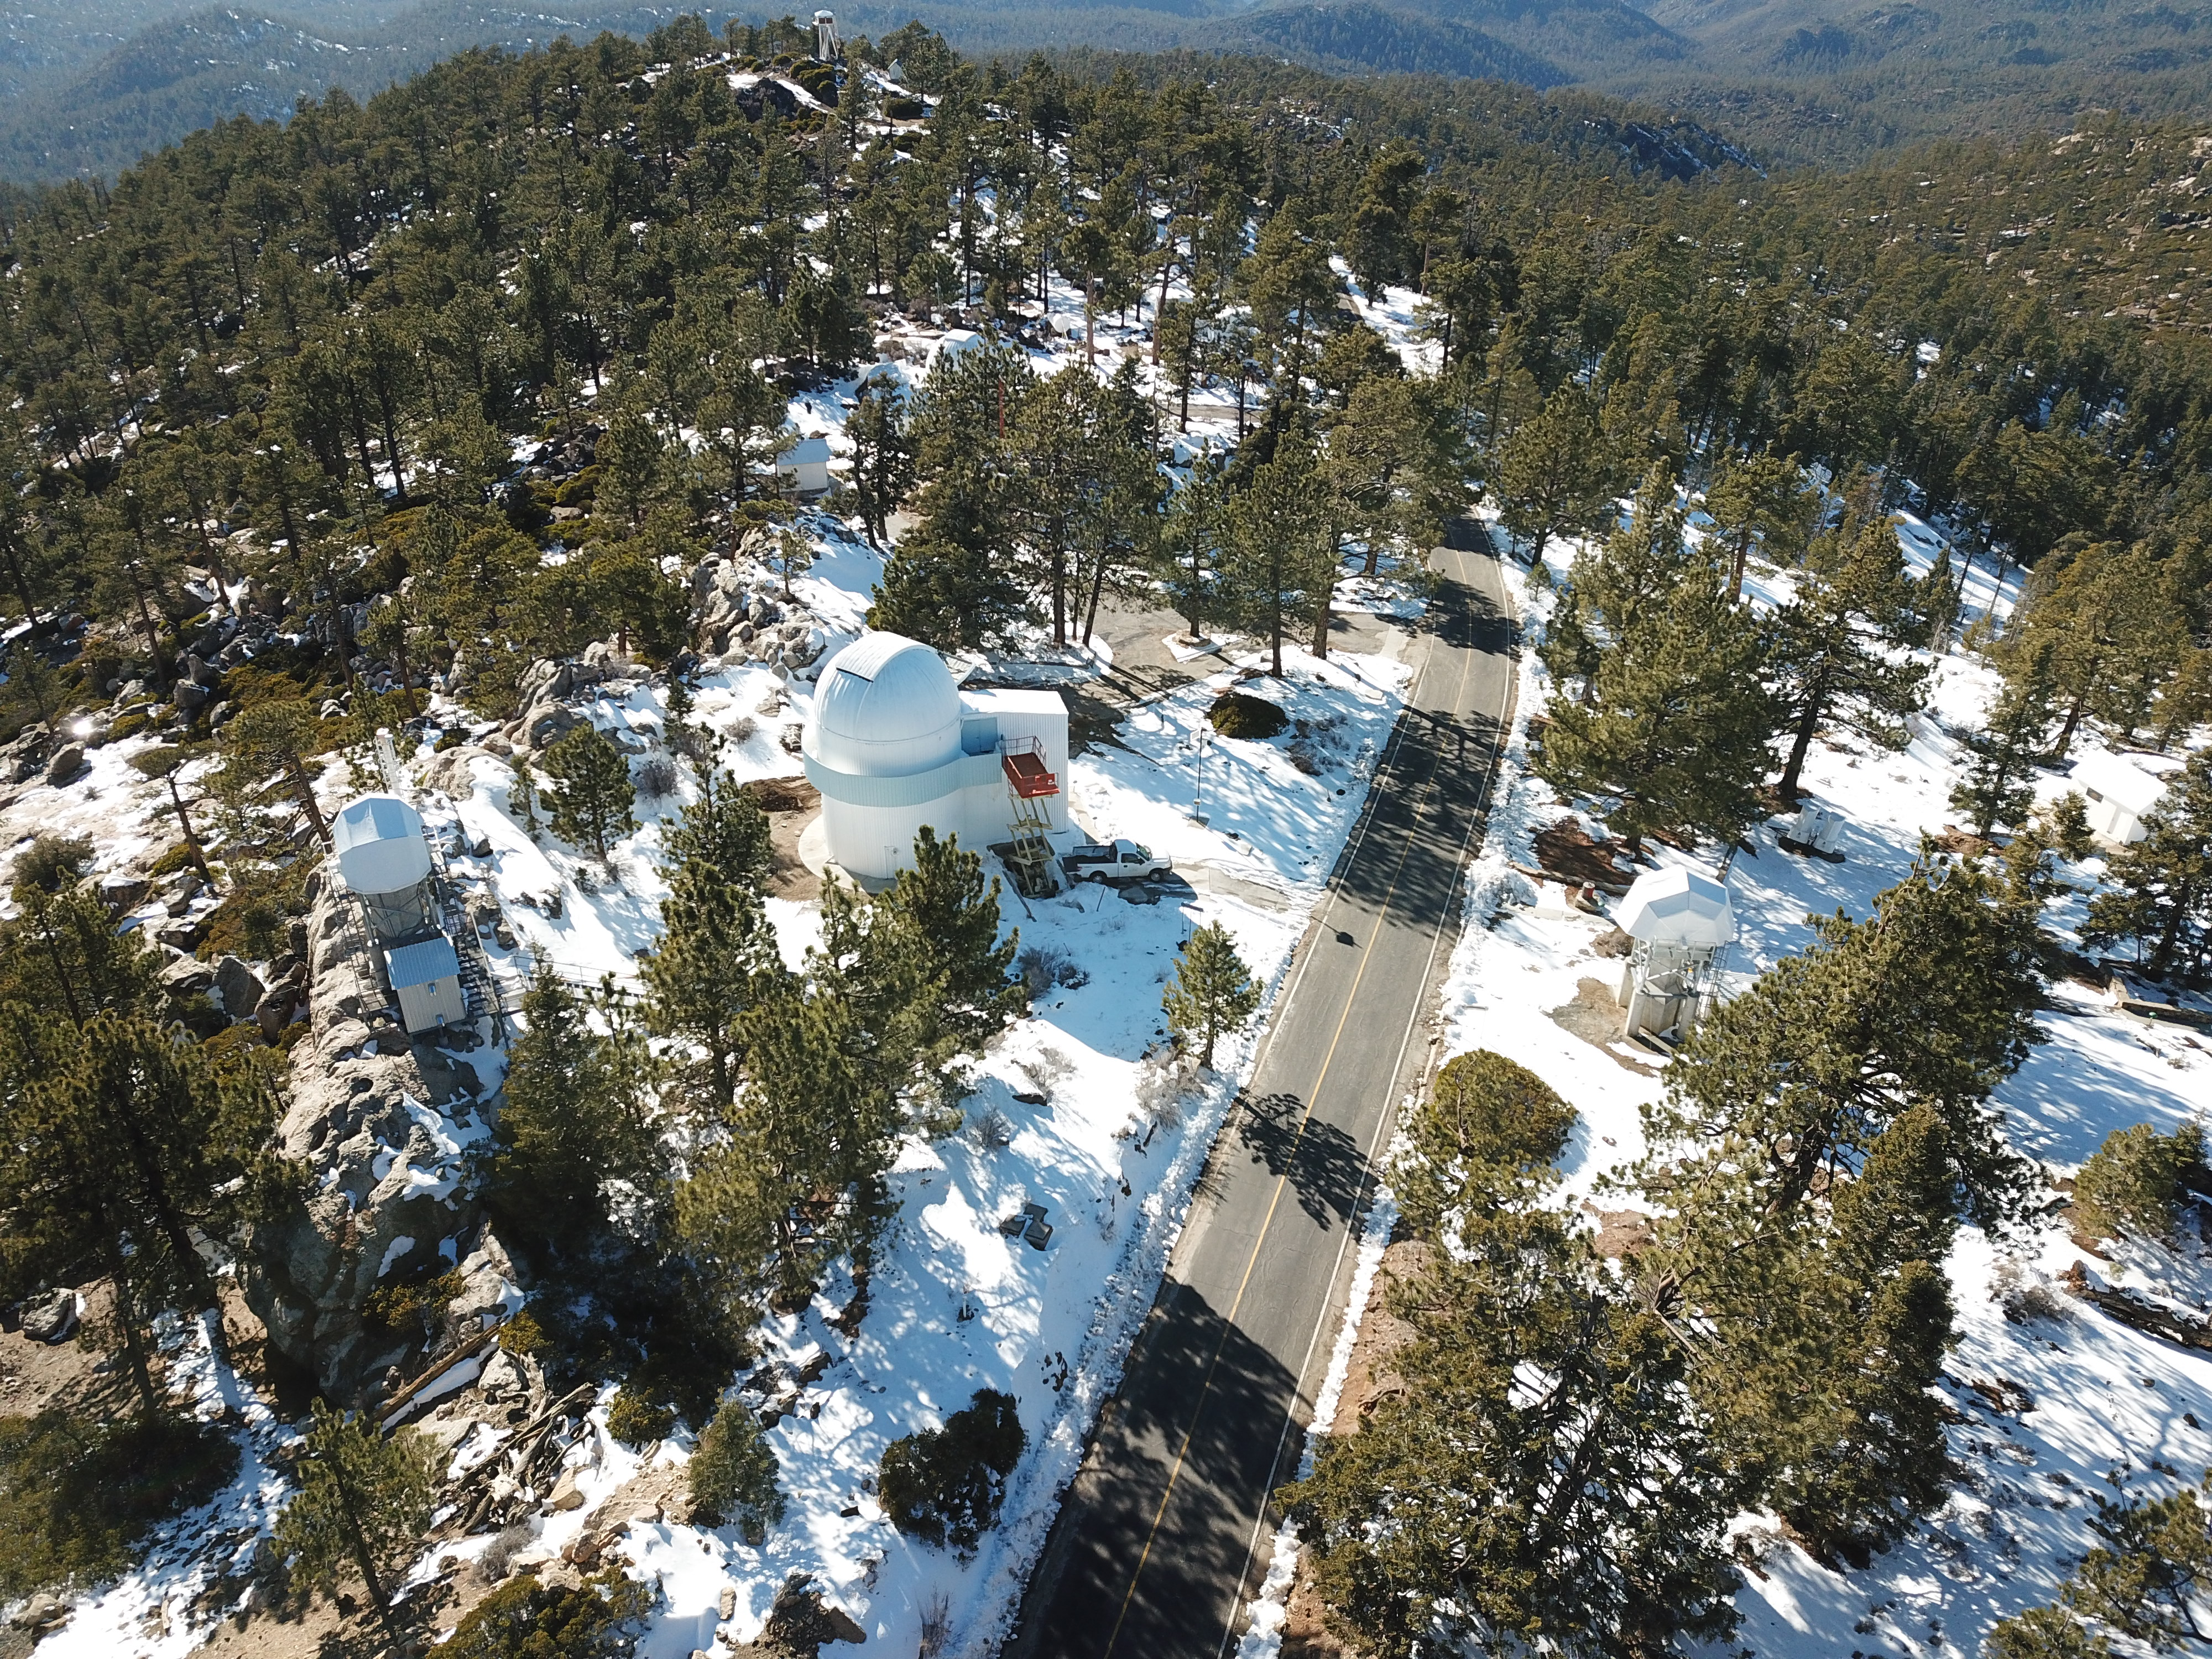
\includegraphics[height=0.7\linewidth]{figures/buildings-general.jpg}
\end{center}
\caption{The COATLI/OAN and DDOTI/OAN installations seen looking west. On the left is the COATLI/OAN shed, access staircase and walkways, tower, platform, and enclosure. In the middle is is 84-cm telescope building. On the right is the DDOTI/OAN tower, platform, enclosure, and shed. Photographer: Fernando Angeles.}
\label{figure:buildings-general}
\end{figure*}


\section{Civil Works}

\ifcoatli

The shed, access, and tower are constructed on a rock outcrop to the south-east of the 84-cm building. The outcrop rises to about 5 meters above the ground level at the 84-cm telescope. The buildings and structures were constructed in 2015--2016, the enclosure was installed in 2016, the enclosure was replaced in 2017, and the telescope column was significantly modified in 2018.

Figures~\ref{figure:buildings-drawing-2015-1} to \ref{figure:buildings-drawing-2015-5} show the 2015 design drawings for the shed, access staircase and walkways, and the concrete columns that support the platform and telescope. Figure  \ref{figure:buildings-drawing-astelco} shows the ASTELCO ARTS platform and the ASTELCO steel pillar mounted on the concrete columns. The center of rotation of the mount axes is 6.5 meters above the rock outcrop and about 11.5 meters above the ground at the 84-cm telescope. The long axis of the enclosure is oriented roughly ENE-WSW to match the shape of the rock outcrop.

The telescope concrete column originally had three parts, each square in cross section and tapering from 1.8, 1.2, and 0.6 meters to a side (see Figure~\ref{figure:buildings-drawing-2015-1}). In 2018, in response to concerns about stiffness, the column was modified and the upper two parts were reinforced to 1.4 meters to a side (see Figure \ref{figure:buildings-drawing-2018-1}). The steel pillar was also filled with concrete to the bottom of the upper holes. The platform floor was modified to accommodate the enlarged column and new support beams for the floor were designed, manufactured, and installed (see Figures \ref{figure:buildings-drawing-2018-2} and \ref{figure:buildings-drawing-2018-3}).

\begin{figure*}
\begin{center}
\includegraphics[height=0.95\linewidth,angle=90]{figures/buildings-coatli-drawing-2015-1.pdf}
\end{center}
\caption{{\projectname} original 2015 design drawing (1 of 5).}
\label{figure:buildings-drawing-2015-1}
\end{figure*}

\begin{figure*}
\begin{center}
\includegraphics[height=0.95\linewidth,angle=90]{figures/buildings-coatli-drawing-2015-2.pdf}
\end{center}
\caption{{\projectname} original 2015 design drawing (2 of 5). The actual stairs turn by 90 degrees to descend towards the 84-cm building. See Figure~\ref{figure:buildings-drawing-2015-3}.}
\label{figure:buildings-drawing-2015-2}
\end{figure*}

\begin{figure*}
\begin{center}
\includegraphics[width=0.95\linewidth]{figures/buildings-coatli-drawing-2015-3.pdf}
\end{center}
\caption{{\projectname} original 2015 design drawing (3 of 5).}
\label{figure:buildings-drawing-2015-3}
\end{figure*}

\begin{figure*}
\begin{center}
\includegraphics[height=0.95\linewidth,angle=90]{figures/buildings-coatli-drawing-2015-4.pdf}
\end{center}
\caption{{\projectname} original 2015 design drawing (4 of 5).}
\label{figure:buildings-drawing-2015-4}
\end{figure*}

\begin{figure*}
\begin{center}
\includegraphics[height=0.95\linewidth,angle=90]{figures/buildings-coatli-drawing-2015-5.pdf}
\end{center}
\caption{{\projectname} original 2018 design drawing (5 of 5).}
\label{figure:buildings-drawing-2015-5}
\end{figure*}

\begin{figure*}
\begin{center}
\includegraphics[height=0.95\linewidth,angle=90]{figures/buildings-coatli-astelco-enclosure-drawing-6610}
\end{center}
\caption{{\projectname} ASTELCO Platform and Telescope Pillar.}
\label{figure:buildings-drawing-astelco}
\end{figure*}

\begin{figure*}
\begin{center}
\includegraphics[height=0.95\linewidth,angle=90]{figures/buildings-coatli-drawing-2018-1.pdf}
\end{center}
\caption{{\projectname} Modified 2018 design drawing (1 of 3).}
\label{figure:buildings-drawing-2018-1}
\end{figure*}

\begin{figure*}
\begin{center}
\includegraphics[height=0.95\linewidth,angle=90]{figures/buildings-coatli-drawing-2018-2.pdf}
\end{center}
\caption{{\projectname} Modified 2018 design drawing (2 of 3).}
\label{figure:buildings-drawing-2018-2}
\end{figure*}

\begin{figure*}
\begin{center}
\includegraphics[height=0.95\linewidth,angle=90]{figures/buildings-coatli-drawing-2018-3.pdf}
\end{center}
\caption{{\projectname} Modified 2018 design drawing (3 of 3).}
\label{figure:buildings-drawing-2018-3}
\end{figure*}
\fi

\ifddoti

The shed, access, and tower are constructed on open space to the north of the 84-cm building. The buildings and structures were constructed in 2016 and the enclosure installed in 2017.

Figures~\ref{figure:buildings-drawing-2016-1} to \ref{figure:buildings-drawing-2016-3} show the 2016 design drawings for the shed, access staircase and walkways, and the concrete columns that support the platform and telescope. The original design was largely based on that of COATLI, but with simplifications for the easier site and a slightly different telescope column. The DDOTI telescope column extended 40 cm above the platform floor (the COATLI column is flush with the platform floor) to reduce the height of the steel pier and increase its stability. Figure  \ref{figure:buildings-drawing-astelco} shows the ASTELCO ARTS platform and the ASTELCO steel pillar mounted on the concrete columns (although this drawing is for COATLI, the DDOTI enclosure is identical except for the perforation in the platform floor). Figure  \ref{figure:buildings-drawing-astelco-pier} shows the ASTELCO pier. The center of rotation of the mount axes is about 6.5 meters above the ground level.

During the summer of 2016, the design of the telescope column was changed without this change being adequately communicated to the project. The telescope concrete column  originally was designed with three parts, each square in cross section and tapering from 1.8, 1.2, and 0.6 meters to a side, like the COATLI column. The design was changed so that the middle and upper sections were uniformly 1.0 meters to a side (although some erroneous vestiges of the original column remain in Figures~\ref{figure:buildings-drawing-2016-1}). Fortunately, this change was caught in time to allow the platform to be modified.

The original design was intended to be oriented with the long-axis of the enclosure aligned with geographic N-S (see Figure~\ref{figure:buildings-drawing-2016-2}). However, when the site was laid out, the surveyor made a sign error in the magnetic deviation. Instead of being aligned with geographic north (11 degrees west of magnetic north) the structures were aligned 22 degrees east of geographic north (11 degrees east of magnetic north). This error was not detected until the lower part of the telescope column had been poured. Fortunately, the column and enclosure could still accommodate the pier, mount, and telescopes.

\begin{figure*}
\begin{center}
\includegraphics[height=0.75\linewidth,angle=90]{figures/buildings-ddoti-drawing-2016-1.pdf}
\end{center}
\caption{{\projectname} original 2016 design drawing (1 of 3).}
\label{figure:buildings-drawing-2016-1}
\end{figure*}

\begin{figure*}
\begin{center}
\includegraphics[height=0.75\linewidth,angle=90]{figures/buildings-ddoti-drawing-2016-2.pdf}
\end{center}
\caption{{\projectname} original 2016 design drawing (2 of 3). Note that the actual installation is rotated approximately 22 degrees east of the orientation shown here.}
\label{figure:buildings-drawing-2016-2}
\end{figure*}

\begin{figure*}
\begin{center}
\includegraphics[height=0.75\linewidth,angle=90]{figures/buildings-ddoti-drawing-2016-3.pdf}
\end{center}
\caption{{\projectname} original 2016 design drawing (3 of 3).}
\label{figure:buildings-drawing-2016-3}
\end{figure*}

\begin{figure*}
\begin{center}
\includegraphics[height=0.75\linewidth,angle=90]{figures/buildings-ddoti-astelco-enclosure-drawing-6610}
\end{center}
\caption{{\projectname} ASTELCO platform and telescope pier (for COATLI).}
\label{figure:buildings-drawing-astelco}
\end{figure*}

\begin{figure*}
\begin{center}
\includegraphics[height=0.75\linewidth,angle=90]{figures/buildings-ddoti-astelco-pier-drawing-3234}
\end{center}
\caption{{\projectname} ASTELCO pier.}
\label{figure:buildings-drawing-astelco-pier}
\end{figure*}

\fi

\section{Ground-Floor of the 84-cm Telescope Building}

We use the ground-floor of the 84-cm telescope building for storage of equipment and as a temporary work space.

{\projectname} tools and equipment are stored mainly in the equipment cabinet. They are to be used only for maintenance of COATLI and DDOTI and must be returned to the cabinet at the end of the maintenance procedure.

ASTELCO tools and equipment are stored in a locked metal box and are only to be used under the supervision of project or ASTELCO personnel.

\section{Shed}
\label{section:shed}
\label{section:shed-key}

The shed contains infrastructure and control electronics.

\begin{figure*}
\begin{center}
\begin{labeled}{\includegraphics[width=0.8\linewidth]{figures/buildings-shed-key.jpg}}
\arrowandlabel{(-1,+3.5)}{(+0,+4)}{west}{Shed Key}
\end{labeled}
\end{center}
\caption{The shed key is hung on the shelves next to the cabinet in the ground floor of the 84-cm telescope building.}
\label{figure:buildings-shed-key}
\end{figure*}

The door to the shed should be left locked. 

The key should be hung on the shelves next to the cabinet in the ground-floor of the 84-cm telescope building (see Figure~\ref{figure:buildings-shed-key}).

The temperature in the shed it controlled by a heater and a pair of fans (one inlet and one exhaust). The fans are controlled by a Lux WIN100 thermostat and are set to turn on at 10 C. The internal thermostat of the heater is set to its minimum level.

%\section{Access Staircase and Walkways}

%\section{Tower, Platform, and Enclosure}

\section{Bibliography}

\begin{flushleft}
\begin{itemize}

\ifcoatli
\item “\href{bibliography/unam-coatli-building-drawing-2015-1.pdf}{Building 2015 Drawing 1 - Columns}”, UNAM.
\item “\href{bibliography/unam-coatli-building-drawing-2015-2.pdf}{Building 2015 Drawing 2 - Plan}”, UNAM.
\item “\href{bibliography/unam-coatli-building-drawing-2015-3.pdf}{Building 2015 Drawing 3 - Stairways}”, UNAM.
\item “\href{bibliography/unam-coatli-building-drawing-2015-4.pdf}{Building 2015 Drawing 4 - Shed}”, UNAM.
\item “\href{bibliography/unam-coatli-building-drawing-2015-5.pdf}{Building 2015 Drawing 5 - Location}”, UNAM.
\item “\href{bibliography/astelco-enclosure-drawing-0500}{ASTELCO Drawing 0500 -- Platform}”, ASTELCO.
\item “\href{bibliography/astelco-enclosure-drawing-5772}{ASTELCO Drawing 5572 -- Tower Mounting Plate}”, ASTELCO.
\item “\href{bibliography/astelco-enclosure-drawing-5772}{ASTELCO Drawing 5798 -- Tower}”, ASTELCO.
\item “\href{bibliography/astelco-enclosure-drawing-5772}{ASTELCO Drawing 6610 --  Tower, Platform, and Enclosure}”, ASTELCO.
\item “\href{bibliography/astelco-enclosure-drawing-5772}{ASTELCO Drawing 6658 -- Tower, Platform, and Enclosuure}”, ASTELCO.
\item “\href{bibliography/astelco-enclosure-drawing-5772}{ASTELCO Drawing 6662 -- Interface}”, ASTELCO.
\item “\href{bibliography/unam-coatli-building-drawing-2018-1.pdf}{Building 2018 Drawing 1 - Column}”, UNAM.
\item “\href{bibliography/unam-coatli-building-drawing-2018-2.pdf}{Building 2018 Drawing 2 - Floor Support Beams}”, UNAM.
\item “\href{bibliography/unam-coatli-building-drawing-2018-3.pdf}{Building 2018 Drawing 3 - Floor Support Beams}”, UNAM.
\fi

\ifddoti
\item “\href{bibliography/unam-ddoti-building-drawing-2016-1.pdf}{Building 2016 Drawing 1 - Columns}”, UNAM.
\item “\href{bibliography/unam-ddoti-building-drawing-2016-2.pdf}{Building 2016 Drawing 2 - Plan and Location}”, UNAM.
\item “\href{bibliography/unam-ddoti-building-drawing-2016-3.pdf}{Building 2015 Drawing 3 - Shed}”, UNAM.
\item “\href{bibliography/astelco-enclosure-drawing-0500}{ASTELCO Drawing 0500 -- Platform}”, ASTELCO.
\item “\href{bibliography/astelco-enclosure-drawing-5772}{ASTELCO Drawing 5572 -- Tower Mounting Plate}”, ASTELCO.
\item “\href{bibliography/astelco-enclosure-drawing-5772}{ASTELCO Drawing 6610 --  Tower, Platform, and Enclosure}”, ASTELCO.
\item “\href{bibliography/astelco-enclosure-drawing-5772}{ASTELCO Drawing 6658 -- Tower, Platform, and Enclosuure}”, ASTELCO.
\item “\href{bibliography/astelco-enclosure-drawing-5772}{ASTELCO Drawing 6662 -- Interface}”, ASTELCO.
\item “\href{bibliography/astelco-ddoti-pier-drawing-3205}{ASTELCO Drawing 3205 -- Pier Mounting Plate}”, ASTELCO.
\item “\href{bibliography/astelco-ddoti-pier-drawing-3205}{ASTELCO Drawing 3234 -- Pier}”, ASTELCO.
\fi

\item “\href{bibliography/lux-win100-manual}{Lux WIN100 Manual}”, Lux.

\end{itemize}
\end{flushleft}

\include{chapter-electrical-power}
\chapter{Electrical Grounding}
\label{chapter:electrical-grounding}

This chapter describes the electrical grounding system in the {\projectname} installation. The electrical power system is described in Chapter~\ref{chapter:electrical-power}.

TODO: Measure DDOTI ground resistance.

\section{Grounding Rods}

\ifcoatli
We have installed a network of ground rods to the 
east of the 84-cm telescope building. There is one main rod and two delta or triad rod systems. The three systems are connected through a ground bar in a box on the eastern wall of the 84-cm telescope.

The 84-cm telescope building is grounded through an independent network of grounding rods just to the south of the building.
\fi

\ifddoti
We have installed a network of ground rods to the 
east of shed. There is one main rod and two delta or triad rod systems. The three systems are connected through a ground bar in a box on the eastern wall of shed.
\fi

TODO: Photo.


\section{Grounding System}

\ifcoatli
Figure~\ref{figure:schematic-electrical-grounding-system} shows a schematic of the electrical grounding system. These grounding cable from the grounding rods runs through the conduit from the 84-cm to the {\projectname} installation. It is terminated at a protected grounding bar underneath the metal walkway. This is the “tau-point” of the grounding system. From here, spurs are used to ground the electrical system in the shed, the walkways, the tower, and the platform.
\fi
\ifddoti
Figure~\ref{figure:schematic-electrical-grounding-system} shows a schematic of the electrical grounding system. These grounding cables from the grounding rods are connected at a protected grounding bar on the east side of the shed. This is the “tau-point” of the grounding system. From here, spurs are used to ground the electrical system in the shed, the tower, and the platform.
\fi

TODO: Photo of the tau-point.

TODO: Cable calibres.

\begin{figure*}
\begin{center}
\resizebox{\columnwidth}{!}{
\begin{tikzpicture}[
 thick,
 box/.style={
  inner sep=1mm,
  draw=black,
  rectangle,
  minimum width=2cm,
  minimum height=0.6cm,
  align=center
 }
] 

\node at (1.5,1.75) [right,align=left] {Ground\\Rods};

\begin{scope}[xshift=0cm,yshift=1.5cm]
\draw (-0.25,-0.0) -- (+0.25,-0.0);
\draw (-0.15,-0.1) -- (+0.15,-0.1);
\draw (-0.05,-0.2) -- (+0.05,-0.2);
\end{scope}
\begin{scope}[xshift=+1cm,yshift=1.5cm]
\draw (-0.25,-0.0) -- (+0.25,-0.0);
\draw (-0.15,-0.1) -- (+0.15,-0.1);
\draw (-0.05,-0.2) -- (+0.05,-0.2);
\end{scope}
\begin{scope}[xshift=-1cm,yshift=1.5cm]
\draw (-0.25,-0.0) -- (+0.25,-0.0);
\draw (-0.15,-0.1) -- (+0.15,-0.1);
\draw (-0.05,-0.2) -- (+0.05,-0.2);
\end{scope}

\draw (-1,1.5) -- (-1,2) -- (0,2);
\draw (+1,1.5) -- (+1,2) -- (0,2);
\draw (0,1.5) -- (0,2);

%\node at (0.2,2) [right] {Conduit};
%\draw (-0.2,1) -- (-0.1,1) -- (-0.1,3) -- (-0.2,3);
%\draw (+0.2,1) -- (+0.1,1) -- (+0.1,3) -- (+0.2,3);

\node (tao-point-ground-bar) at (0,4) [box,minimum width=11cm] {Tau-Point Ground Bar};

\draw (0,2) -- (tao-point-ground-bar);

\ifcoatli
\node (walkways) [box] at (-4.5,5.5) {Walkways};
\draw ($(tao-point-ground-bar.north) + (-4.5,0)$) -- (walkways);
\fi

\node (shed-ground-bar) at (-1.5,7.5) [box,minimum width=5 cm] {Shed Ground Bar};
\draw ($(tao-point-ground-bar.north) + (-1.5,0)$) -- (shed-ground-bar);

\node (tower) [box] at (+1.5,5.5) {Tower};
\draw ($(tao-point-ground-bar.north) + (+1.5,0)$) -- (tower);

\node (platform-ground-bar) at (4.5,11.5) [box,minimum width=5 cm] {Platform Ground Bar};
\draw ($(tao-point-ground-bar.north) + (+4.5,0)$) -| (platform-ground-bar.south);

\node (circuit-box) [box] at (-3.0,8.5) {Circuit Box};
\draw ($(shed-ground-bar.north) + (-1.5,0)$) -- (circuit-box.south);

\node (circuits-a-f) [box] at (-3.0,9.5) {Circuits A--F};
\draw (circuit-box) -- (circuits-a-f);

\node (rack-chassis) [box] at (+0.0,8.5) {Rack Chassis};
\draw ($(shed-ground-bar.north) + (+1.5,0)$) -- (rack-chassis.south);

\node (box-b) [box] at (3.0,12.5) {Power Box};
\draw ($(platform-ground-bar.north) + (-1.5,0)$) -- (box-b.south);

\ifcoatli
\node (boxes) [box] at (3.0,13.5) {Platform/Instrument Boxes};
\fi
\ifddoti
\node (boxes) [box] at (3.0,13.5) {Platform/Detectors Boxes};
\fi
\draw (box-b) -- (boxes);

\node (mount) [box] at (6.0,12.5) {Mount};
\draw ($(platform-ground-bar.north) + (+1.5,0)$) -- (mount.south);

\draw[dashed] (-6,6.5) -- (+8,6.5);
\draw[dashed] (-6,10.5) -- (+8,10.5);
\draw[dashed] (-6,14.5) -- (+8,14.5);
\node at (-6,+8.5) [right] {\normalsize Shed};
\node at (-6,+12.5) [right] {\normalsize Platform};

\end{tikzpicture}
}
\end{center}
\caption{Schematic of the Electrical Grounding System}
\label{figure:schematic-electrical-grounding-system}
\end{figure*}

The ground bar in the shed is used to provide ground to circuit box and hence to the circuits and the sockets in the shed. It is also used to ground the rack.

Circuits B1, B2, and C run from the shed to Box B on the platform. However, their ground is not connected in Box B. Instead, the ground bar on the platform is used to provide ground for Box B and subsequently for the sockets on the platform (in boxes B and C), the cables to boxes C, D, E, and F, and the mount.

TODO: Make sure the ground is connected to the cables between the boxes.

The Astelco controllers in the shed are connected to the platform and mount. There are undoubtedly ground loops through these connections. However, the connections from the platform to the tau-point is through a heavy-gauge cable, and this is likely to mitigate these ground loops.

\ifcoatli

\section{Ground Resistance}

In October 2016 we measured a ground resistance of about 5.5~$\Omega$ at all three of the ground bars (the tau-point, shed ground bar, and platform ground bar) using the three-point method. We further measured a resistance of about 0.8~$\Omega$ between the grounding point of the NTM-500 mount and the platform grounding bar and between the ground contacts of the outlets of the iBootBars and the shed grounding bar. This suggests that the grounding system is working well.

\fi

\chapter{Network}
\label{chapter:network}

TODO: haltsoon and rebootsoon

\begin{figure*}
\begin{center}
\resizebox{!}{0.9\textheight}{
\begin{tikzpicture}
[
 thick,
 box/.style={
  draw,
  minimum height=1cm,
  minimum width=2cm,
  inner sep=1mm,
  align=center,
 }
]
 \footnotesize
 \node at (0,0) (internet) [box] {Internet};
 
 \draw[dashed] (-4.5,1.0) -- (+4.5,1.0) -- (+4.5,6.0) -- (-4.5,6.0) -- node [above,rotate=90] {84-cm} cycle;

 \node at (0,2.0) (oan-firewall) [box] {OAN/SPM\\Firewall};
 \ifcoatli
 \node at (3,3.5) (webcam-c) [box] {webcam-c\\132.148.4.16};
 \fi
 \ifddoti
 \node at (3,3.5) (webcam-c) [box] {webcam-c\\132.148.4.26};
 \fi
 \node at (0,3.5) (switch-84) [box] {Switch\\84-cm};
 \node at (0,5.0) (fiber-84) [box] {Fibre Adapter};
 
 \draw (internet) -- (oan-firewall);
 \draw (switch-84) -- (webcam-c);
 \draw (oan-firewall) -- (switch-84);
 \draw (switch-84) -- (fiber-84);

 \draw[dashed] (-4.5,6.5) -- (+4.5,6.5) -- (+4.5,13.0) -- (-4.5,13.0) -- node [above,rotate=90] {Shed} cycle;
 
 \node at (0,7.5) (firewall) [box] {10.0.1.1\\firewall\\{\projectexternalipaddress}};
 \node at (0,9.75) (switch-rack) [box] {Switch\\Rack};

 \draw (fiber-84) -- (firewall);
 \draw (firewall) -- (switch-rack);

 \node at (-3,12.0) (console) [box] {console\\10.0.1.2};
 \node at (-3,10.5) (control) [box] {control\\10.0.1.9};
 \node at (-3,9.0) (airport0) [box] {airport0\\10.0.1.30};
 \node at (+3,12.0) (ibb-220) [box] {ibb-220\\10.0.1.4}; 
 \node at (+3,10.5) (ibb-127) [box] {ibb-127\\10.0.1.5}; 
 \node at (+3,9.0) (mount) [box] {mount\\10.0.1.6};
 \node at (+3,7.5) (serial) [box] {serial\\10.0.1.7};
 
 \draw (switch-rack) -- (console);
 \draw (switch-rack) -- (airport0);
 \draw (switch-rack) -- (control);
 \draw (switch-rack) -- (ibb-127);
 \draw (switch-rack) -- (ibb-220);
 \draw (switch-rack) -- (mount);
 \draw (switch-rack) -- (serial);
 
 \draw[dashed] (-4.5,13.5) -- (+4.5,13.5) -- (+4.5,17.0) -- (-4.5,17.0) -- node [above,rotate=90] {Platform} cycle;

 \node at (0,15.25) (switch-platform) [box] {Switch\\Platform Box};
 \node at (-3,14.5) (platform) [box] {platform\\10.0.1.10}; 
 \node at (-3,16.0) (airport1) [box] {airport1\\10.0.1.31}; 
 \node at (+3,14.5) (webcam-a) [box] {webcam-a\\10.0.1.20}; 
 \node at (+3,16.0) (webcam-b) [box] {webcam-b\\10.0.1.21}; 
 \draw (switch-platform) -- (platform);
 \draw (switch-rack) -- (switch-platform);
 \draw (switch-platform) -- (webcam-a);
 \draw (switch-platform) -- (webcam-b);
 \draw (switch-platform) -- (airport1);
 
 \ifcoatli 
 \draw[dashed] (-4.5,17.5) -- (+4.5,17.5) -- (+4.5,19.5) -- (-4.5,19.5) -- node [above,rotate=90] {Telescope} cycle;
 \node at (-3,18.5) (instrument) [box] {instrument\\10.0.1.12}; 
 \node at (+3,18.5) (ib-detector) [box] {ib-detector\\10.0.1.11}; 
 \draw (switch-platform) -- (ib-detector);
 \draw (switch-platform) -- (instrument);
 \fi

 \ifddoti 
 \draw[dashed] (-4.5,17.5) -- (+4.5,17.5) -- (+4.5,21.0) -- (-4.5,21.0) -- node [above,rotate=90] {Telescope} cycle;
 \node at (-3,18.5) (detectors0) [box] {detectors0\\10.0.1.11}; 
 \node at (0,18.5) (switch-detectors0) [box] {Switch\\Detectors 0 Box};
 \draw (switch-platform) -- (switch-detectors0);
 \draw (switch-detectors0) -- (detectors0);
 \node at (-3,20.0) (detectors1) [box] {detectors1\\10.0.1.12}; 
 \node at (0,20.0) (switch-detectors1) [box] {Switch\\Detectors 1 Box};
 \draw (switch-detectors0) -- (switch-detectors1);
 \draw (switch-detectors1) -- (detectors1);
 \fi
 
\end{tikzpicture}
}
\end{center}
\caption{Network Physical Topology}
\label{figure:network-topology}
\end{figure*}

\section{WAN and LAN Addresses}

The observatory uses 132.248.4.0/24 as a WAN. {\projectname} uses 10.0.1.0/24 as a LAN. The firewall computer in the rack in the shed serves as a firewall and router between the WAN and the LAN. The addresses of the equipment are given in Table~\ref{table:network-addresses}.

\begin{table*}
\caption{Addresses}
\label{table:network-addresses}
\begin{center}
%\footnotesize
\begin{tabular}{llll}
\hline
Address&Name&Equipment&Location\\
\hline
{\projectexternalipaddress}&\verb|firewall|&Ubiquiti Edgerouter X-SFP&Rack\\
10.0.1.1&\verb|firewall|&Ubiquiti Edgerouter X-SFPr&Rack\\
10.0.1.2&\verb|console|&Raspberry Pi 4&Rack\\
10.0.1.4&\verb|ibb-220|&iBootBar 220 V&Rack\\
10.0.1.5&\verb|ibb-127|&iBootBar 127 V&Rack\\
10.0.1.6&\verb|mount|&Mount Controller&Rack\\
10.0.1.7&\verb|serial|&Serial Adapter&Shed Wall\\
10.0.1.9&\verb|control|&HP Server Server&Rack\\
10.0.1.10&\verb|platform|&Raspberry Pi 4&Platform Box\\
\ifcoatli
10.0.1.11&\verb|ib-detector|&iBoot&Platform\\
10.0.1.12&\verb|instrument|&Kingsdel PC&Instrument Box\\
\fi
\ifddoti
10.0.1.11&\verb|detectors0|&Kingsdel PC&Detectors 0 Box\\
10.0.1.12&\verb|detectors1|&Kingsdel PC&Detectors 1 Box\\
\fi
10.0.1.20&\verb|webcam-a|&Webcam&Platform (above Power Box)\\
10.0.1.21&\verb|webcam-b|&Webcam&Platform (above Platform Box)\\
10.0.1.30&\verb|airport0|&Airport Express&Rack\\
10.0.1.31&\verb|airport1|&Airport Express&Platform Box\\
10.0.1.200 to 10.0.1.250&DHCP\\
\ifcoatli
132.248.4.16&\verb|webcam-c|&Webcam&84-cm (SE side)\\
\fi
\ifddoti
132.248.4.26&\verb|webcam-c|&Webcam&84-cm (NE side)\\
\fi
\hline
\end{tabular}
\end{center}
\end{table*}

\section{Port Filtering and Forwarding}

The observatory firewall filters access to {\ttfamily \projectexternalipname} ({\projectexternalipaddress}) from outside the observatory WAN except for ports TCP/22 (SSH), TCP/80 (HTTP), and \ifcoatli
TCP/5349 (GCN/TAN).
\fi
\ifddoti
TCP/5351 (GCN/TAN).
\fi

The firewall forwards certain TCP ports from its WAN address to hosts on the LAN. These are listed in Table~\ref{table:port-forwarding}. The firewall restricts access on most of these port, with only the main ssh port being open to all hosts.

\begin{table}
\caption{Ports Forwarded from the WAN to the LAN}
\label{table:port-forwarding}
\begin{center}
\begin{tabular}{llll}
\hline
Port on WAN&Host on LAN&Port on LAN&Notes\\
\hline
22&\verb|access|&22&Main ssh access.\\
80&\verb|services|&80&Web page and interface.\\
873&\verb|services|&5349&rsync.\\
2222&\verb|firewall|&22&Backup ssh access.\\
\ifcoatli
5349&\verb|services|&5349&GCN/TAN notices.\\
\fi
\ifddoti
5351&\verb|services|&5351&GCN/TAN notices.\\
\fi
\hline
\end{tabular}
\end{center}
\end{table}

\section{Access}

All of the hosts have an account {\projectaccount} with password {\projectaccount}. Local and ssh access is permitted on the Linux machines, but only local access is permitted on the \verb|access|.

SSH access to \verb|access| is limited to the accounts of project staff and the OAN/SPM network maintenance staff. Thus, remote access is accomplished by first logging into \verb|access| using a non-{\projectaccount} account and then logging into a local machine using the {\projectaccount} account.

We recommend using an \href{https://help.ubuntu.com/community/SSH/OpenSSH/Keys}{SSH public key} to avoid needing to type passwords repeatedly. If you do not have a key, you can generate one by running these commands on your computer:
\begin{verbatim}
mkdir ~/.ssh
chmod 700 ~/.ssh
ssh-keygen -t rsa
\end{verbatim}
Once you have generated a key, you can copy it to \verb|access| using:
\ifcoatli
\begin{verbatim}
ssh-copy-id user@coatli.astrossp.unam.mx
\end{verbatim}
\fi
\ifddoti
\begin{verbatim}
ssh-copy-id user@ddoti.astrossp.unam.mx
\end{verbatim}
\fi
You should then by able to ssh to \verb|access| without having to type your password.

Having copied the key to access, you can copy it to the {\projectaccount} accounts on the other computers on the LAN by running this command on \verb|access|:
\begin{verbatim}
ssh-copy-id-to-lan
\end{verbatim}
To use your key this, you should make sure that the key is forwarded by using the \verb|-A| option to ssh when you connect to \verb|access| or by adding the \verb|ForwardAgent yes| option to your \verb|.ssh/config| file.

\section{Wireless Networks}

There are two wireless networks for general use. 
\ifcoatli
The access Mac in the shed implements \verb|apcoatli0| and the Airport Extreme in Box C on the platform implements \verb|apcoatli1|. 
\fi
\ifddoti
The access Mac in the shed implements \verb|apddoti0| and the Airport Extreme in Box C on the platform implements \verb|apddoti1|. 
\fi
The password is “keplerxv”.

\section{DHCP}

The firewall runs a DHCP server that allocates addresses in the range 10.0.1.100 to 10.0.1.200.


\chapter{Lights}
\label{chapter:lights}

This chapter describes the lighting in the {\projectname} installation. 

\section{Shed Lights}

The shed has standard manual lights controlled by a switch just inside the door. 

The shed lights are on circuit E and are backed up by emergency lighting that switches on if the power fails.

\section{Platform Manual Lights}

The platform manual lights controlled by a switch on Box B by the usual entrance to the platform. The lights are a small LED panel supplied by a 12~VDC power supply in Box B.

The platform manual lights are on circuit C and are backed up by emergency lighting that switches on if the power fails.
 
\section{Platform Remote-Controlled Lights}

\subsection{Hardware}

The platform remote-controlled lights controlled by Box C. The lights are a small LED panel supplied by a 12~VDC power supply in Box C. Electrically, the supply is switched by a H-bridge controlled by GPIO pin 481 on \verb|c0|.

The platform remote-controlled lights are on circuit B1.

\subsection{Control}

The \verb|lights| server for the remote-controlled lights runs on \verb|c0|.

The server starts automatically after \verb|c0| boots, but if necessary it can be stopped, started, or restarted explicitly by issing the following shell commands on \verb|c0|:

\begin{itemize}
\item sudo stopserver lights
\item sudo startserver lights
\item sudo restartserver lights
\end{itemize}

Server requests can be issued from any of the Mac or Linux machines on the LAN. The following requests are supported:

\begin{itemize}
\item 
\verb|request lights status|

Show the status of the server.

Obtain the values of the status data from the server and print them to stdout.
\item 
\verb|request lights initialize|

Initialize the server and hardware. As part of the process of initializing, the lights will switch off.

\item 
\verb|request lights reset|

Attempt to recover from an error.

\item 
\verb|request lights stop|

Attempt to stop the current activity.

\item 
\verb|request lights switchon|

Switch the lights on.

\item 
\verb|request lights switchoff|

Switch the lights off.

\end{itemize}

There are buttons to control the lights on the web interface. These are useful for illuminating the platform to allow inspection by the webcams.

\chapter{Webcams}
\label{chapter:webcams}

TODO: Photos of the webcams.

TODO: Photos with the webcams.

{\projectname} uses webcams to monitor the platform and enclosure from inside and out.

\begin{figure}[t]
\begin{center}
\ifcoatli
\includegraphics[height=0.6\linewidth]{figures/coatli-webcam-a.jpg}
\fi
\ifddoti
\includegraphics[height=0.6\linewidth]{figures/ddoti-webcam-a.jpg}
\fi
\end{center}
\caption{Typical daytime view from {\projectname} webcam A.}
\label{figure:webcam-a-view}
\begin{center}
\ifcoatli
\includegraphics[height=0.6\linewidth]{figures/coatli-webcam-b.jpg}
\fi
\ifddoti
\includegraphics[height=0.6\linewidth]{figures/ddoti-webcam-b.jpg}
\fi
\end{center}
\caption{Typical daytime view from {\projectname} webcam B.}
\label{figure:webcam-b-view}
\end{figure}

\begin{figure}[t]
\begin{center}
\ifcoatli
\includegraphics[height=0.6\linewidth]{figures/coatli-webcam-c.jpg}
\fi
\ifddoti
\includegraphics[height=0.6\linewidth]{figures/ddoti-webcam-c.jpg}
\fi
\end{center}
\caption{Typical daytime view from {\projectname} webcam C.}
\label{figure:webcam-c-view}
\begin{center}
\ifcoatli
\includegraphics[height=0.6\linewidth]{figures/coatli-webcam-cz.jpg}
\fi
\ifddoti
\includegraphics[height=0.6\linewidth]{figures/ddoti-webcam-cz.jpg}
\fi
\end{center}
\caption{Typical daytime view from {\projectname} webcam CZ (en electronic zoom of webcam C).}
\label{figure:webcam-cz-view}
\end{figure}

\section{Platform Webcams}

There are two webcams installed on short posts on the platform. Webcam A is installed above Box B and webcam B is installed above Box C. Figures~\ref{figure:webcam-a-view} and \ref{figure:webcam-b-view} show typical daytime views from webcams A and B. Between them, they can see all of the platform. The platform remote light allow the webcams to monitor the platform even at night. The webcams are Vivotek FE8174V with a 180 degree field of view. This model has an IP66-rated weatherproof housing and can operate down to $-40$~C.

The platform webcams are on the LAN at the addresses given in Table~\ref{table:network-addresses}. The web interfaces can be accessed with the “\projectaccount” account with password “\projectaccount”.

\section{External}

Webcam C is installed on the outside wall of the 84-cm, above the balcony, giving a view of the {\projectname} enclosure. An electronic zoom of webcam C, that shows the enclosure in more detail, is known as webcam CZ. Figures~\ref{figure:webcam-c-view} and \ref{figure:webcam-cz-view} show typical daytime views from webcams C and CZ.
The webcam is a Vivotek MD7560D with a $98 \times 73$ degree field of view lens. This model has an IP67-rated weatherproof housing and can operate down to $-25$~C.

The external webcam in on the observatory public network at the address given in Table~\ref{table:network-addresses}. The web interfaces can be accessed with the “\projectaccount” account with password “\projectaccount”.

\section{Bibliography}

\begin{flushleft}
\begin{itemize}
\item “\href{bibliography/vivotek-fe8174v-data-sheet.pdf}{FE8174/74V Data Sheet}”, Vivotek.
\item “\href{bibliography/vivotek-fe8174v-manual.pdf}{FE8174V User’s Manual}”, Vivotek.
\item “\href{bibliography/vivotek-md7560-alignment-sticker.pdf}{MD7530/60 MD8562/62D Alignment}”, Vivotek.
\item “\href{bibliography/vivotek-md7560-data-sheet.pdf}{MD7560/60D Data Sheet}”, Vivotek.
\item “\href{bibliography/vivotek-md7560-manual.pdf}{MD7530/7530D MD7560/7560D User’s Manual}”, Vivotek.
\item “\href{bibliography/vivotek-md7560-quick-instaltion-guide.pdf}{MD7530/7530D MD7560/7560D Quick Installation Guide}”, Vivotek.
\end{itemize}
\end{flushleft}

\include{chapter-enclosure}

\include{part-telescope-and-instrument}

\include{chapter-mount}
\include{chapter-telescope-coatli}
\include{chapter-secondary-coatli}
% !TEX root = coatli.tex

\chapter{The Huitzi $f/20$ Imager}

The Huitzi $f/20$ imager was installed on the COATLI telescope in December 2022. The imager is named for the mexica god \href{https://en.wikipedia.org/wiki/Huītzilōpōchtli}{Huītzilōpōchtli}, the son of the goddess Coatlicue.

Earlier, the “Interim Imager” and “Huitzi $f/8$ Imager” were installed on the telescope. For historical reference, these are described in Appendices~\ref{appendix:interim-imager} and \ref{appendix:instrument-huitzi-f8}.

\section{Overview}

\begin{figure*}[p]
\begin{center}
\includegraphics[width=0.7\linewidth]{figures/huitzi-f20-on-telescope.jpg}
\medskip
\caption{The Huitzi $f/20$ imager on the COATLI telescope.}
\label{figure:huitzi-f20-on-coatli}
\end{center}
\end{figure*}

Figure~\ref{figure:huitzi-f20-on-coatli} shows the Huitzi $f/20$ imager on the telescope.

The imager uses a 150 mm diverging lens to convert the $f/8$ beam of the telescope into an $f/20$ beam. This beam is then imaged an Andor iXon electron-multiplying CCD detector with $1024\times1024$ pixels with a pixel scale of 0.27 arcsec and a field of 4.6 arcmin. The detector can be read through either a conventional amplifier or the electron-multiplying amplifier at a variety of speeds.

The imager has three Finger Lakes Instruments filter wheels. Currently, the following filters can be provided:

\begin{itemize}
\item open: Completely open.
\item dark: Completely blocked.
\item $grizy$: Filters similar to the Pan-STARRS equivalents. Note, however, that while the filters are similar, the CCD is not deep-depleted and so the bandpasses are somewhat different.
\item $w$: A filter that combines the $r$ and $i$ bands. Note that this is different to Pan-STARRS $w$ which includes the $g$ band too. It is mainly intended for sensitive imaging of GRBs.
\item $BVRI$: Johnson-Cousins filters according to the Bessell formulation.
\item $\Is$: The $I$ filter with a sharp red cutoff at 900 nm. This is intended to better match the bandpass of the original Cousins (1978) $I$ photomety. The blue edge is the same as the Bessell formulation, but the red edge is defined by a 900 nm short-pass filter to simulate the red edge of a GaAs tube. The Bessell (1990) and Bessell \& Murphy (2012) bandpasses fall at about 900 nm.
\item 470/10, 515/10, and 640/10: Nebular continuum filters.
\item 501/8, 656/3, 656/8: Nebular line filters.
\end{itemize}

Some of these filters are constructed from combinations of filters in different wheels, as described in more detail below.

The detector is mounted on Optec Gemini focuser and rotator, which allows up to 12.7 mm of motion of the detector with respect to the lens.

\section{Optics}

\begin{figure*}[t]
\begin{center}
\resizebox{0.9\linewidth}{!}{
\begin{tikzpicture}
\draw[dashed](-10,0) -- (12,0);
\draw(-8,+2) -- (-4,+1);
\draw(-8,-2) -- (-4,-1);
\draw[dotted](-4,+1) -- (0,0) -- (-4,-1);
\draw[>-<] (-4,-2) -- (-4,+2);
\draw (-4,+1) -- (10,0) -- (-4,-1);
\draw (-4,-2.5) node {$S$};
\draw (0,-2.5) node {$A$};
\draw (10,-2.5) node {$A'$};
\end{tikzpicture}
}
\end{center}
\medskip
\caption{Schematic of the Optical Design}
\label{figure:huitzi-f20-optical-design}
\end{figure*}

The effect of the negative lens is shown schematically in Figure~\ref{figure:huitzi-f20-optical-design}. $A$ is the position of the telescope focus without the lens. $S$ is the position of the lens. $A'$ is the position of the telescope focus with the lens. 
The magnification $m$ is given by
$$
	m = SA'/SA,
$$
in which $SA'$ and $SA$ are optical distances.
If the focal length of the lens is $F$, then Gauss’ equation gives the relation between $SA$ and $SA'$ as:
$$
	1/F = 1/SA' - 1/SA.
$$
We then solve to find:
$$
	m = 1 - SA'/F
$$
and
$$
	SA' = - (m - 1) F.
$$
We can see the approximate dimensions of the system by ignoring chromatic aberration and taking $F = -150$ mm. Then, if we choose $SA = 90$ mm we have $SA' = 225$ mm and $m = 2.5$. Since the focal ratio of the telescope is $f/8$, this magnification gives a focal ratio of $f/20$.

\begin{figure*}
\begin{center}
\includegraphics[angle=90,width=0.9\linewidth]{figures/huitzi-f20-lens-design.pdf}
\medskip
\caption{The lens design.}
\label{figure:huitzi-f20-lens-design}
\end{center}
\end{figure*}

The actual lens is Edmund Optics part \#63-767, whose design is shown in Figure~\ref{figure:huitzi-f20-lens-design}. It has a design effective focal length of $-150$ mm at 587.6 nm. It is nominally 40 mm in diameter and 13.54 mm thick at the edge. The precise optical and mechanical prescriptions of are given in the files “\verb|zmax_63767.ZMX|”and “\verb|step_63767.STP|” supplied by Edmund Optics. The lens is used with the convergent element B uppermost (towards the secondary) and the divergent element A lowermost (towards the detector). That is, surface S4 is uppermost (towards the secondary) and surface S1 is lowermost (towards the detector). If the lens is inverted, the system will suffer significant spherical aberration.

The lens is an achromatic doublet, so its focal length varies with wavelength. This has two effects. First, the different focal length between bands requires us to refocus for each filter. In theory, we could adjust both the secondary and the focuser to achieve focus while holding the magnification constant. In practice, we simply adjust the focuser to maintain focus and let the magnification vary slightly. (The focuser is also used to compensate for the different optical thicknesses of the filters.) Second, chromatic aberration within the $g$ and $B$ bands limits their image quality.

The lens has a $\lambda/4$ MgF$_2$ coating on both surfaces.

The lens also serves as a window to prevent ingress of dust and insects.

\section{Filters}

The upper filter wheel (“A”) is an FLI CFW-1-5 wheel for five 50 mm diameter filters. The two lower filter wheels (“B” and “C”) are FLI CFW-1-8 wheels for eight 25 mm diameter filters. The elements installed in each wheel are shown in Table~\ref{table:huitzi-f20-filter-wheel-loading}.

\begin{table*}
\begin{center}
\caption{Filter Wheel Loading}
\label{table:huitzi-f20-filter-wheel-loading}
\medskip
\begin{tabular}{lccc}
\hline
Slot&A&B&C\\
\hline
0&open	&P0			&open		\\
1&$B$	&656/3		&$g$		\\
2&$V$	&470/10		&$r$		\\
3&$R$	&$z$			&$i$		\\
4&825SP	&$I$			&550LP	\\
5&			&925LP		&900SP	\\
6&			&515/10		&656/8	\\
7&			&640/10		&501/8	\\
\hline
\end{tabular}
\end{center}
\end{table*}

The filter elements are:

\begin{itemize}
\item $griz$: These are similar to the Pan STARRS filters. They were acquired from Custom Scientific and fabricated to our specifications. They are 25 mm in diameter and 5 mm thick. They have dielectric coatings on fuzed silica substrates.
\item $BVRI$: These are Johnson-Cousins filters adapted from the Bessell (1990) recipe. They are off-the-shelf filters acquired from Custom Scientific. They are 50 mm ($BVR$) or 25 mm ($I$) diameter and 5 mm thick.
From modeling the transmission curves, we believe the recipes are:
\begin{itemize}
\item $B$: 2 mm Hoya L38 + 1 mm Schott BG25 + 2 mm Schott BG39
\item $V$: 1 mm Schott GG495 + 3 mm Schott BG39 + 1 mm filler
\item $R$: 2 mm Schott OG570 + 3 mm Schott KG3
\item $I$: 3 mm Schott RG9 + 2 mm filler
\end{itemize}
\item 825SP: This is an 825 nm OD4 short-pass filter. It is Edmund Optics part \#86-113. It is 50 mm in diameter and 5 mm thick. It has  dielectric coatings on a fuzed silica substrate.
\item 925LP: This is an 925 nm OD4 long-pass filter. It is Edmund Optics part \#86-072. It is 25 mm in diameter and 3 mm thick. It has  dielectric coatings on a fuzed silica substrate.
\item 900SP: This is an 900 nm OD4 short-pass filter. It is Edmund Optics part \#64-335. It is 25 mm in diameter and 3 mm thick. It has  dielectric coatings on a fuzed silica substrate.
\item 550LP: This is an 550 nm OD4 long-pass filter. It is Edmund Optics part \#62-984. It is 25 mm in diameter and 3 mm thick. It has dielectric coatings on a fuzed silica substrate.
\item P0: This is a window. It is Edmund Optics part \#48-066. It is 25 mm in diameter and 3 mm thick. It has Edmund UV-VIS coatings on a fused silica substrate.
\item 470/10, 501/8, 515/10, 640/10, 656/3, and 656/8: These are narrow-band filters, named for their approximate central wavelength and width in nm. They are off-the-shelf filters acquired from Custom Scientific. They are 25 mm in diameter and 3 mm thick. They have dielectric coatings on a fuzed silica substrate.

\begin{figure}
\begin{center}
\includegraphics[width=0.7\linewidth]{figures/huitzi-f20-damaged-470-10-filter.jpg}
\medskip
\caption{The damaged 470/10 filter.}
\label{figure:huitzi-f20-damaged-470-10-filter}
\end{center}
\end{figure}

The 470/10 filter was damaged in April 2023. The central screw in wheel A came loose, jammed in filter wheel B, and scratched the 470/10 filter. Figure~\ref{figure:huitzi-f20-damaged-470-10-filter}. We are seeking to buy a replacement.

In addition to these, we have 486/8 and 501/3 filters that could be installed by special request. Furthermore, Custom Scientific have 672/3, 672/8, and 889/18 filters that could be purchased for about US\$500 each.
\end{itemize}

\begin{table*}
\begin{center}
\caption{Filter Combinations}
\label{table:huitzi-f20-filter-combinations}
\medskip
\begin{tabular}{lcccc}
\hline
Filter&A&B&C&Thickness (mm)\\
\hline
dark		&$B$		&$z$		&656/8	&\phantom{}13		\\
open		&open		&P0		&open		&\phantom{0}3		\\
$g$		&open		&P0		&$g$		&\phantom{0}8		\\
$r$		&open		&P0		&$r$		&\phantom{0}8		\\
$i$			&open		&P0		&$i$		&\phantom{0}8		\\
$z$		&open		&$z$		&open		&\phantom{0}5		\\
$y$		&open		&925LP	&550LP	&\phantom{0}6		\\
$w$		&825SP	&P0		&550LP	&\phantom{}11		\\
$B$		&$B$		&P0		&open		&\phantom{0}8		\\
$V$		&$V$		&P0		&open		&\phantom{0}8		\\
$R$		&$R$		&P0		&open		&\phantom{0}8		\\
$I$		&open		&$I$		&open		&\phantom{0}5		\\
$\Is$		&open		&$I$		&900SP	&\phantom{0}8		\\
470/10	&open		&470/10	&open		&\phantom{0}3		\\
501/8		&open		&P0		&501/8	&\phantom{0}6		\\
515/10	&open		&515/10	&open		&\phantom{0}3		\\
640/10	&open		&640/10	&open		&\phantom{0}3		\\
656/3		&open		&656/3	&open		&\phantom{0}3		\\
656/8		&open		&P0		&656/8	&\phantom{0}6		\\
\hline
\end{tabular}
\end{center}
\end{table*}

The filter bandpasses are created by combinations of conventional bandpass filters, long-pass, and short-pass filters. The combinations used are given in Table~\ref{table:huitzi-f20-filter-combinations}. Most of the combinations are straightforward, but we comment on three aspects in particular:

\begin{itemize}
\item $\Is$: The system responses in both $I$ and $\Is$ have their blue edge defined by RG9 glass. However, in $I$ the red edge is defined by the CCD but in $\Is$ (“$I$ short”) it is defined by the 900SP filter. This gives $\Is$ a system response that is a better match that of Cousins (1978), whose $I$ has its the red edge defined by the cutoff of a GaAs photocathode around 900 nm. Compare Figure~\ref{figure:huitzi-f20-S-JC-IIs} here with Figure~9 of Bessell \& Murphy (2012).

\item
$w$: The $w$ filter essentially encompasses the bandpasses of $r$ and $i$ (although the exact edges are slightly different). Note that this is different to Pan-STARRS $w$ which includes the $g$ band too. It is mainly intended for sensitive imaging of GRBs.

\item P0: The role of the P0 (“prism 0”) element might seem to be a puzzle. However, we are considering converting the telescope to an altitude-azimuth configuration at some point in the future and installing wedged windows P1 and P2, similar to P0, in wheel B in place of two of the narrow-band filters. This will allow us to implement an atmospheric dispersion corrector  for the $BVR$ and $griw$ filters using P0, P1, and P2. However, while the telescope is in an equatorial configuration, there is no point in installing P1 and P2. We could have left the position occupied by P0 as open, but we decided to install it to give consistent bandpasses in these filters in both the equatorial and altitude-azimuth configurations.

\end{itemize}

Model system efficiency curves at the zenith (including the atmosphere, telescope mirrors, lens, filters, detector window, and detector, but excluding the obscuration of the secondary) are shown in Figures~\ref{figure:huitzi-f20-S-first} to \ref{figure:huitzi-f20-S-last}.

\begin{figure*}
\begin{center}
\includegraphics[width=0.7\linewidth]{figures/huitzi-f20-S-grizy.png}
\medskip
\caption{The model system efficiency $S$ at the zenith in the $grizy$ filters. The dotted line is the model unfiltered efficiency.}
\label{figure:huitzi-f20-S-first}
\end{center}
\end{figure*}

\begin{figure*}
\begin{center}
\includegraphics[width=0.7\linewidth]{figures/huitzi-f20-S-w-open.png}
\medskip
\caption{The model system efficiency $S$ at the zenith in the $w$ and open filters. The dotted line is the model unfiltered efficiency.}
\end{center}
\end{figure*}

\begin{figure*}
\begin{center}
\includegraphics[width=0.7\linewidth]{figures/huitzi-f20-S-JC-BVRI.png}
\medskip
\caption{The model system efficiency $S$ at the zenith in the $BVRI$ filters. The dotted line is the model unfiltered efficiency.}
\end{center}
\end{figure*}

\begin{figure*}
\begin{center}
\includegraphics[width=0.7\linewidth]{figures/huitzi-f20-S-JC-IIs.png}
\medskip
\caption{The model system efficiency $S$ at the zenith in the $I$ and $\Is$ filters. The $\Is$ filter has a red cutoff defined by the 900SP filter whereas the $I$ filter has the red cutoff defined by the CCD. The dotted line is the model unfiltered efficiency.}
\label{figure:huitzi-f20-S-JC-IIs}
\end{center}
\end{figure*}

\begin{figure*}
\begin{center}
\includegraphics[width=0.7\linewidth]{figures/huitzi-f20-S-g.png}
\medskip
\caption{The model system efficiency $S$ at the zenith in the $g$ filter.}
\end{center}
\end{figure*}

\begin{figure*}
\begin{center}
\includegraphics[width=0.7\linewidth]{figures/huitzi-f20-S-r.png}
\medskip
\caption{The model system efficiency $S$ at the zenith in the $r$ filter.}
\end{center}
\end{figure*}

\begin{figure*}
\begin{center}
\includegraphics[width=0.7\linewidth]{figures/huitzi-f20-S-i.png}
\medskip
\caption{The model system efficiency $S$ at the zenith in the $i$ filter.}
\end{center}
\end{figure*}

\begin{figure*}
\begin{center}
\includegraphics[width=0.7\linewidth]{figures/huitzi-f20-S-z.png}
\medskip
\caption{The model system efficiency $S$ at the zenith in the $z$ filter.}
\end{center}
\end{figure*}

\begin{figure*}
\begin{center}
\includegraphics[width=0.7\linewidth]{figures/huitzi-f20-S-y.png}
\medskip
\caption{The model system efficiency $S$ at the zenith in the $y$ filter.}
\end{center}
\end{figure*}

\begin{figure*}
\begin{center}
\includegraphics[width=0.7\linewidth]{figures/huitzi-f20-S-w.png}
\medskip
\caption{The model system efficiency $S$ at the zenith in the $w$ filter.}
\end{center}
\end{figure*}

\begin{figure*}
\begin{center}
\includegraphics[width=0.7\linewidth]{figures/huitzi-f20-S-open.png}
\medskip
\caption{The model system efficiency $S$ at the zenith in the open filter.}
\end{center}
\end{figure*}

\begin{figure*}
\begin{center}
\includegraphics[width=0.7\linewidth]{figures/huitzi-f20-S-JC-B.png}
\medskip
\caption{The model system efficiency $S$ at the zenith in the $B$ filter.}
\end{center}
\end{figure*}

\begin{figure*}
\begin{center}
\includegraphics[width=0.7\linewidth]{figures/huitzi-f20-S-JC-V.png}
\medskip
\caption{The model system efficiency $S$ at the zenith in the $V$ filter.}
\end{center}
\end{figure*}

\begin{figure*}
\begin{center}
\includegraphics[width=0.7\linewidth]{figures/huitzi-f20-S-JC-R.png}
\medskip
\caption{The model system efficiency $S$ at the zenith in the $R$ filter.}
\end{center}
\end{figure*}

\begin{figure*}
\begin{center}
\includegraphics[width=0.7\linewidth]{figures/huitzi-f20-S-JC-I.png}
\medskip
\caption{The model system efficiency $S$ at the zenith in the $I$ filter.}
\end{center}
\end{figure*}

\begin{figure*}
\begin{center}
\includegraphics[width=0.7\linewidth]{figures/huitzi-f20-S-JC-Is.png}
\medskip
\caption{The model system efficiency $S$ at the zenith in the $\Is$ filter.}
\end{center}
\end{figure*}

\begin{figure*}
\begin{center}
\includegraphics[width=0.7\linewidth]{figures/huitzi-f20-S-NBMB.png}
\medskip
\caption{The model system efficiency $S$ at the zenith in the narrow-band and medium-band filters. The dotted line is the model unfiltered efficiency.}
\end{center}
\end{figure*}

\begin{figure*}
\begin{center}
\includegraphics[width=0.7\linewidth]{figures/huitzi-f20-S-NBMB-g.png}
\medskip
\caption{The model system efficiency $S$ at the zenith in the narrow-band and medium-band filters in $g$: 470/10, 486/8, 501/3, 501/8, and 515/10. The filters shown with dashed lines have not yet been acquired. The dotted line is the model unfiltered efficiency. The blue vertical lines are at 486.1, 495.9, and 500.7 nm.}
\end{center}
\end{figure*}

\begin{figure*}
\begin{center}
\includegraphics[width=0.7\linewidth]{figures/huitzi-f20-S-NBMB-r.png}
\medskip
\caption{The model system efficiency $S$ at the zenith in the narrow-band and medium-band filters in $r$: 640/10, 656/3, 656/8, 672/3, and 672/8, 501/8, and 515/10. The filters shown with dashed lines have not yet been acquired. The dotted line is the model unfiltered efficiency. The blue vertical lines are at 656.3, 654.8, 658.4, 671.6, and 673.1 nm.}
\end{center}
\end{figure*}

\begin{figure*}
\begin{center}
\includegraphics[width=0.7\linewidth]{figures/huitzi-f20-S-NBMB-z.png}
\medskip
\caption{The model system efficiency $S$ at the zenith in the medium-band filter in $z$: 889/18. The filters shown with dashed lines have not yet been acquired. The dotted line is the model unfiltered efficiency.}
\label{figure:huitzi-f20-S-last}
\end{center}
\end{figure*}

\begin{table*}
\begin{center}
\caption{Model Filter Properties}
\label{table:huitzi-f20-model-filter-properties}
\medskip
\begin{tabular}{lccc}
\hline
Filter&$\lambda_\mathrm{pivot}$ (nm)&$\Delta\lambda$ (nm)&ZP ($\mathrm{s}^{-1}$)\\
\hline
open		& 618.7& \phantom{}384.1&$4.2 \times 10^{9}$\\
$g$		& 475.9& \phantom{}104.6&$1.2 \times 10^{9}$\\
$r$		& 617.2& \phantom{}132.4&$1.3 \times 10^{9}$\\
$i$			& 747.4& \phantom{}131.5&$8.0 \times 10^{8}$\\
$z$		& 862.8& \phantom{0}94.8&$3.0 \times 10^{8}$\\
$y$		& 973.3& \phantom{0}64.2&$8.6 \times 10^{7}$\\
$w$		& 668.4& \phantom{}264.6&$2.2 \times 10^{9}$\\
$B$		& 446.5& \phantom{0}89.4&$5.9 \times 10^{8}$\\
$V$		& 537.9& \phantom{0}89.8&$8.5 \times 10^{8}$\\
$R$		& 633.9& \phantom{}118.0&$1.0 \times 10^{9}$\\
$I$		& 814.8& \phantom{}150.7&$8.0 \times 10^{8}$\\
$\Is$		& 795.0& \phantom{}150.7&$7.0 \times 10^{8}$\\
470/10	& 469.7& \phantom{0}10.1&$9.9 \times 10^{7}$\\
486/8		& 485.5& \phantom{00}9.3&$1.0 \times 10^{8}$\\
501/3		& 500.7& \phantom{00}3.2&$3.5 \times 10^{7}$\\
501/8		& 500.5& \phantom{00}7.0&$8.2 \times 10^{7}$\\
515/10	& 514.2& \phantom{0}10.0&$1.1 \times 10^{8}$\\
640/10	& 638.9& \phantom{00}9.9&$9.8 \times 10^{7}$\\
656/3		& 656.5& \phantom{00}2.9&$2.8 \times 10^{7}$\\
656/8		& 655.9& \phantom{00}7.7&$8.4 \times 10^{7}$\\
672/3		& 672.3& \phantom{00}2.9&$2.7 \times 10^{7}$\\
672/8		& 672.2& \phantom{00}7.6&$6.8 \times 10^{7}$\\
889/18	& 887.3& \phantom{0}17.5&$4.3 \times 10^{7}$\\
\hline
\end{tabular}
\end{center}
\end{table*}

Table~\ref{table:huitzi-f20-model-filter-properties} gives the model properties of the filter. The filter pivot wavelength $\lambda_\mathrm{pivot}$ is  defined by 
$$
\lambda_\mathrm{pivot} \equiv \sqrt{\frac{\int \lambda S\,d\lambda}{\int S/\lambda\, d\lambda}}.
$$
For a discussion of the interpretation of the pivot wavelength, see \S A2.1 of Bessell \& Murphy (2012).
The filter FWHM is defines as the width over which $S$ is at least half its maximum. The filter ZP is the expected electron count rate for a star with AB = 0,
$$
ZP \equiv A \int S F_\lambda / (hc/\lambda)\, d\lambda,
$$
in which $A$ is the geometric area of the telescope (the area of the primary mirror not occulted by the secondary obscuration) and $F_\lambda$ is the flux density of a source with $F_\nu = \mathrm{3631~Jy}$.

We are monitoring photometric standards from Oke \& Gunn (1983) to verify the theoretical zero-points and sensitivity curves presented above. Initial results suggest that the zero points in the blue are approximately correct, but beyond about 600 nm the observed sensitivity is only about 75\% of the theoretical sensitivity.

\section{Focuser and Rotator}

The instrument incorporates an Optec Gemini focuser and rotator between the last filter wheel and the detector.

The focuser moves from 0 to 115200 steps over 12.7 mm which corresponds to 9.07 steps per micron. The 0 position is above and the 115200 position is below. The focuser moves at about 900 steps or 0.1 mm per second.

\section{Focus Compensation}

The lens has chromatic aberration and the filters have different thicknesses. Both of these require us to use a compensator to maintain focus. Our options are the focuser, the secondary, or both. If we use only one compensator, then the magnification necessarily changes slightly was we adjust for focus. If we use both, we can maintain the magnification. 

However, it is fairly easy to show that if we use the focuser, either on its own or in combination with the secondary to maintain the magnification, in the worst case we need to move it about 3 mm. Since the focuser moves at about 0.1 mm per second, this means the worse case time is about 30 seconds. This is long compared to slew speed (without a meridian flip) and cannot be overlapped with changing the filter.  On the other hand, if we use only the secondary, in the worst case we need to move about 60 steps. Even with backlash compensation, this takes about 5.5 seconds. Furthermore, this can be overlapped with changing the filter. Therefore, in the interests of preserving the rapid response of COATLI, we have chosen to compensate the focus using only the secondary. This compensation is handled automatically by the control system.

Our model is as follows. We define $L$ to be the (fixed) physical distance from the lens to the detector and $T$ to be the total physical thickness of filter glass between the lens and the detector. We then have
$$
SA' = L - [(n - 1) / n] T \approx L - 0.32 T,
$$
where we have assumed $n = 1.48$ for fused silica. We then solve for SA using
$$
1/F = 1/SA' - 1/SA,
$$
taking into account the dependence of $F$ on wavelength. We determine $\Delta SA$ relative to the $i$ filter. We then determine the corresponding change in the secondary taking into account the amplification of 10.64 between the movement of the secondary and the movement of the telescope focal plane.

Table \ref{table:huitzi-f20-filter-secondary-offsets} shows the results. Note that for the medium band filters, there are two values depending on whether the filter is in wheel B ($T = 3$ mm) or wheel C ($T = 6$ mm). The offsets of the narrowband filters are the same as for the corresponding medium band filters.

\begin{table*}
\begin{center}
\caption{Filter Secondary Offsets}
\label{table:huitzi-f20-filter-secondary-offsets}
\medskip
\begin{tabular}{lccc}
\hline
Filter&$F$ (mm)&Thickness (mm)&Offset (steps)\\
\hline
open		&$-150.22$		&\phantom{0}3		&\phantom{}$-24$\\
$g$		&$-150.20$		&\phantom{0}8		&\phantom{0}$+7$\\
$r$		&$-150.07$		&\phantom{0}8		&\phantom{}$+13$\\
$i$			&$-150.37$		&\phantom{0}8		&\phantom{+0}$0$\\
$z$		&$-150.66$		&\phantom{0}5		&\phantom{}$-30$\\
$y$		&$-150.96$		&\phantom{0}6		&\phantom{}$-37$\\
$w$		&$-150.25$		&\phantom{}11		&\phantom{}$+24$\\
$B$		&$-150.43$		&\phantom{0}8		&\phantom{0}$-2$\\
$V$		&$-150.97$		&\phantom{0}8		&\phantom{}$+17$\\
$R$		&$-150.14$		&\phantom{0}8		&\phantom{}$+10$\\
$I$		&$-150.27$		&\phantom{0}5		&\phantom{}$-30$\\
$\Is$		&$-150.50$		&\phantom{0}8		&\phantom{0}$-5$\\
470/10	&$-149.99$		&\phantom{}3/6		&\phantom{}$-14/+4$\\
515/10	&$-149.93$		&\phantom{}3/6		&\phantom{}$-12/+6$\\
640/10	&$-150.07$		&\phantom{}3/6		&\phantom{}$-16/+1$\\
\hline
\end{tabular}
\end{center}
\end{table*}

\section{Detector}

The detector unit is an Andor iXon Ultra 888 with an e2v CCD201-20 electron-multiplying CCD detector. The detector was acquired in 2014 and originally intended to be the tilt sensor for the planned two-channel imager.

\subsection{Format, Scale, and Field}

The detector has $1024\times1024$ pixels each $13\times13$ {\micron} square. 

The detector gives a pixel scale of 0.269 arcsec and a field of 4.59 arcmin. 

\begin{figure*}
\begin{center}
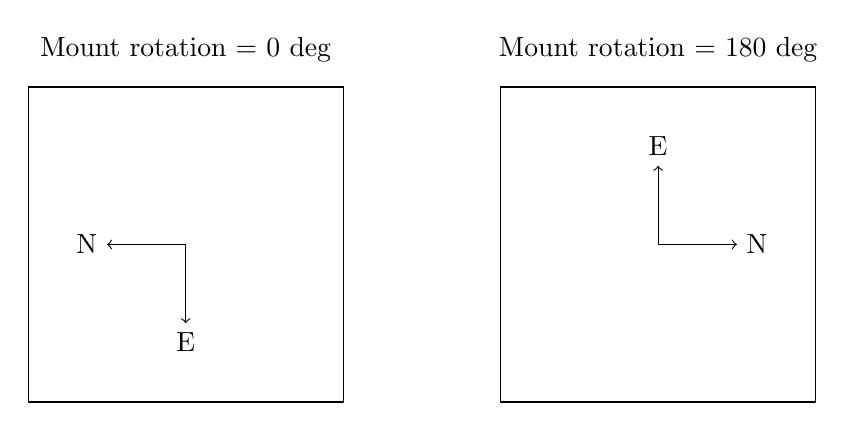
\begin{tikzpicture}
\begin{scope}[xshift=-3cm]
\draw (-2,-2) -- (+2,-2) -- (+2,+2) -- (-2,+2) -- cycle;
\draw (0,2.2) node [anchor=south] {Mount rotation = 0 deg};
\draw[->] (0,0) -- (-1,0) node [anchor=east] {N};
\draw[->] (0,0) -- (0,-1) node [anchor=north] {E};
\end{scope}
\begin{scope}[xshift=3cm]
\draw (-2,-2) -- (+2,-2) -- (+2,+2) -- (-2,+2) -- cycle;
\draw (0,2.2) node [anchor=south] {Mount rotation = 180 deg};
\draw[->] (0,0) -- (1,0) node [anchor=west] {N};
\draw[->] (0,0) -- (0,1) node [anchor=south] {E};
\end{scope}
\end{tikzpicture}
\end{center}
\caption{The orientation of the detector on the sky according to the mount rotation. The pixel origin is in the lower left.}
\label{figure:huitzi-f20-detector-orientation}
\end{figure*}

The orientation of the field on the sky depends on the mount rotation (given by the values of the \verb|SMTMRO| and \verb|EMTMRO| keywords in the header), and is shown in Figure~\ref{figure:huitzi-f20-detector-orientation}. However, the pipeline reduction rotates all images to the conventional orientation with north up and east left.

\subsection{Quantum Efficiency}

The detector has standard silicon and the e2v midband coating (which in Andor's terminology makes it a “BV” device). The nominal quantum efficiency is shown in Figure~\ref{figure:huitzi-f20-detector-quantum-efficiency}. The detector has excellent efficiency from 500 to 800 nm.

\begin{figure*}
\begin{center}
\begin{tikzpicture}
\small
\begin{axis}[
   xmin=300,
   xmax=1100,
   xlabel={$\lambda$ (nm)},
   xticklabel style={
     /pgf/number format/precision=0,
     /pgf/number format/fixed,
     /pgf/number format/fixed zerofill
   },
   minor x tick num=3,
   ymin=0,
   ymax=1,
   minor y tick num=3,
   ylabel={$\eta$},
   legend style={
     cells={anchor=west},
     legend pos=north east,
   },
]
\addplot [black] table [x=lam, y=Q, col sep=comma] {figures/huitzi-detector-efficiency.csv};
\end{axis}
\end{tikzpicture}
\end{center}
\caption{The nominal quantum efficiency $\eta$ of the Huitzi detector.}
\label{figure:huitzi-f20-detector-quantum-efficiency}
\end{figure*}

\subsection{Readout Architecture}

The detector can be read using either a conventional signal chain (at 100 kHz or 1 MHz) or an EM signal chain (at 1, 10, 20, or 30 MHz). Both chains have two gains and the EM gain can be set to up to 1000. 

Although the conventional and EM amplifiers clock the serial register in different directions, the control software flips each row in conventional data so that physical pixels have the same logical position in the FITS files.

The detector is used in frame-transfer mode without a mechanical shutter (see \S\ref{section:huitzi-f20-shutter}). At the end of an exposure, the charge is rapidly clocked into from the light-sensitive image section to the shielded store section. The change can then be read. In EM mode, the next exposure can then start immediately.

With the normal vertical-shift frequency of 4.33 MHz, the frame transfer takes about 4.5 ms. This leads to some trailing above and below bright stars.

The read-out architecture has several parameters, which are encoded in the value of the \verb|READMODE| header keyword. The value is a string of the form $A$-$B$-$C$-$D$-$E$-$F$-$G$ in which $A$ to $G$ are non-negative integers with the following meanings:

\begin{itemize}
\item[$A$] The ADC channel index. This is always 0 since the detector only has one ADC channel.
\item[$B$] The amplifier index. This is 0 for the EM amplifier and 1 for the conventional amplifier.
\item[$C$] The vertical shift speed index. For both amplifiers, 0 is 0.60 MHz, 1 is 1.13 MHz, 2 is 2.20 MHz, and 3 is 4.33 MHz. 
\item[$D$] The horizontal shift speed index. For the EM amplifier, 0 is 30 MHz, 1 is 20 MHz, 2 is 10 MHz, and 3 is 1 MHz. For the conventional amplifier, 0 is 1 MHz and 1 is 100 kHz.
\item[$E$] The gain index. For both amplifiers, 0 is low gain (more electrons per ADU) and 1 is high gain (fewer electrons per ADU).
\item[$F$] The nominal EM gain. This is ignored when the conventional amplifier is used. For the EM amplifier, it can be between 1 and 1000.
\item[$G$] The software gain. After the data are read, each ADU signal is divided by the software gain to reduce white noise in the low-order bits (see \href{https://ui.adsabs.harvard.edu/abs/2002RMxAA..38..233W/abstract}{Watson 2002, RMAA, 38, 233}).
\end{itemize}

Fortunately, there is little need to use these values directly, since aliases are defined for common modes. They are shown in Table~\ref{table:huitzi-f20-read-mode-aliases}.

\begin{table*}
\caption{Read-Mode Aliases}
\label{table:huitzi-f20-read-mode-aliases}
\begin{center}
\begin{tabular}{lll}
\hline
Alias&Mode\\
\hline
 initial&default\\
 default&em-30MHz\\
 conventionaldefault&1MHz\\
 fastguidingdefault&em-30MHz\\
 1MHz&1MHz-low\\
 em-10MHz&em-10MHz-low\\
 em-20MHz&em-20MHz-low\\
 em-30MHz&em-30MHz-low\\
 1MHz-low&0-1-3-0-0-1-1\\
 1MHz-high&0-1-3-0-1-1-2\\
 em-10MHz-low&0-0-3-2-0-250-2\\
 em-10MHz-high&0-0-3-2-1-160-4\\
 em-20MHz-low&0-0-3-1-0-500-4\\
 em-20MHz-high&0-0-3-1-1-320-8\\
 em-30MHz-low&0-0-3-0-0-1000-8\\
 em-30MHz-high&0-0-3-0-1-640-16\\
 \hline
\end{tabular}
\end{center}
\end{table*}

\subsection{Shutter and Dark Filter}

\label{section:huitzi-f20-shutter}

We originally attempted to use the mechanical shutter for conventional CCD modes and the frame-transfer capability for EM modes. However, we found that the shutter sometimes failed to open or failed to open completely. We suspect that at the colder temperatures of winter nights night, the power supply does not provide sufficient voltage to open the shutter.  

Therefore, we now leave the shutter open between exposures and use the frame-transfer capability in both conventional and EM modes. As noted above, with the normal vertical-shift frequency, the frame transfer takes about 4.5 ms.

Note that the shutter closes when the detector head is powered down. This sometimes occurs at night, as the detector head sometimes becomes uncommunicative and is automatically powered down and up again by the control system. There is a risk that after such a cycle the shutter will not open or not open completely.

To take bias and dark images, we have use a “dark” filter that consists of the $B$, $z$, and 656/8 filters in series. Despite this, light leaks in the filter wheel mean that we need to take biases and darks at night.

\begin{table*}
    \centering
    \begin{tabular}{lcccc}
    \hline
    Mode Name&1MHz-0&em-10MHz-0&em-20MHz-0&em-30MHz-0\\
    \hline
    Amplifier&Conventional&EM&EM&EM\\
    Horizontal Speed&1 MHz&10 MHz&20 MHz&30 MHz\\
    Software Gain&1&2&4&8\\
    ADC Range (DN)&64k&32k&16k&8k\\
    Gain ($e^-$/DN)&3.3&41&78&117\\
    Read Noise (DN)&2.1&2.6&1.9&1.7\\
    Read Noise ($e^-$)&7&105&145&204\\
    Bias Level (DN)&500&242&123&62\\
    Linear Limit ($e^-$)&&400k&400k&400k\\
    Saturation (DN)&58k&32k&16k&8k\\
    Saturation ($e^-$)&190k&1300k&1250k&940k\\
    Linearity ($e^-$)&&400k&400k&400k\\
    Linearity (DN)&&9700&5100&3400\\
    Dynamic Range (bits)&&11.9&11.4&10.9\\
    \hline
    \end{tabular}
    \caption{Detector Characteristics with the Low Preamplifier Gain}
    \label{table:huitzi-f20-detector-characteristics-low-gain}
\end{table*}

\begin{table*}
    \centering
    \begin{tabular}{lcccc}
    \hline
    Mode Name&1MHz-1&em-10MHz-1&em-20MHz-1&em-30MHz-1\\
    \hline
    Amplifier&Conventional&EM&EM&EM\\
    Horizontal Speed&1 MHz&10 MHz&20 MHz&30 MHz\\
    Software Gain&2&4&8&16\\
    ADC Range (DN)&32k&16k&8k&4k\\
    Gain ($e^-$/DN)&1.6&21&45&70\phantom{0}\\
    Read Noise (DN)&2.9&2.7&2.4&1.6\\
    Read Noise ($e^-$)&5&56&108&115\\
    Bias Level (DN)&250&119&62&31\\
    Saturation (DN)&22k&\\
    Saturation ($e^-$)&35k&\\
    Linearity ($e^-$)&&400k&400k&400k\\
    Linearity (DN)&&19000&8900&5700\\
    Dynamic Range (bits)&&12.8&11.9&11.8\\
    \hline
    \end{tabular}
    \caption{Detector Characteristics with the High Preamplifier Gain}
    \label{table:huitzi-f20-detector-characteristics-high-gain}
\end{table*}

\section{Mechanics}

\begin{table*}
\caption{Mechanical Parts and Hardware}
\medskip
\footnotesize
\begin{center}
\begin{tabular}{llll}
\hline
part&Name&Quantity&Notes\\
\hline
1&Instrument flange&1\\
2&Main barrel&1\\
3&Lens barrel ring&1\\
4&Lens barrel&1&Edmund Optics \#57-978\\
5&Upper filter wheel interface plate&1\\
6&Filter wheel&3&FLI CFW-1-5 (A) or CFW-1-8 (B and C)\\
7&Filter wheel separator&2\\
8&Lower filter wheel interface plate&1\\
9&Upper focuser interface ring&1\\
10&Focuser&1&Optec Gemini\\
11&Lower focuser interface ring&1\\
12&Detector head&1&Andor iXon Ultra 888\\
13&Detector posts&2&Andor 12.7 mm diameter 80 mm long with 1/4-20 thread\\
14&Detector cable support plate&1\\
X&Lens barrel separator&1\\
?&Filter wheel adapter&2&FLI part supplied with filter wheels\\
Z&Internal baffle&2&Black nylon\\
\hline
15&SS Hex Head Screw M5×0.8×12&12&McMaster 91287A122\\
16&SS Belleville Spring Lock Washer M5&12&McMaster 90895A027\\
17&Threaded Insert M5×0.8×7.5&12&McMaster 97120A220 (= part 22)\\
18&Threaded rod M3×0.5&6&Modified from McMaster 90024A218\\
19&SS Hex Nut M3×0.5&6&McMaster 91828A211\\
20&SS Spring Lock Washer Conical M3&6&McMaster 91477A121\\
21&Thread-Lock Insert M3×0.5×6.5&6&McMaster 97120A190\\
22&Threaded Insert M5×0.8×7.5&4&McMaster 97120A220 (= part 17)\\
23&SS Socket Head Screw M5×0.8×10&8&McMaster 91292A124\\
24&SS Oval-Tip Set Screw 18-8 1/4-inch&6&McMaster 92778A113\\
25&SS Flat-Tip Set Screw 18-8 1/8-inch&6&McMaster 94355A180\\
26&SS Hex Socket Screw Flat Head 82 deg Countersink 1/4-20 1/2-inch&2&McMaster 92210A537\\
27&SS Belleville Spring Lock Washer 1/4&2&McMaster 93501A029\\
28&SS Hex Socket Screw Button Head M5×0.8×50&4&McMaster 92095A228\\
?&Hex Socket Screw M5×0.8&6&\\
\hline
\end{tabular}
\end{center}
\end{table*}

\begin{figure*}
\begin{center}
\includegraphics[angle=180,width=0.9\linewidth]{figures/huitzi-f20-3d.pdf}
\end{center}
\caption{The instrument mechanics.}
\label{figure:huitzi-f20-3d}
\end{figure*}

\begin{figure*}
\begin{center}
\includegraphics[angle=180,width=0.9\linewidth]{figures/huitzi-f20-3d-exploded.pdf}
\end{center}
\caption{The instrument mechanics (exploded view).}
\label{figure:huitzi-f20-3d-exploded}
\end{figure*}

\begin{figure*}
\begin{center}
\includegraphics[angle=180,width=0.9\linewidth]{figures/huitzi-f20-section.pdf}
\end{center}
\caption{The instrument mechanics (longitudinal section).}
\label{figure:huitzi-f20-section}
\end{figure*}

\begin{figure*}
\begin{center}
\includegraphics[angle=180,width=0.9\linewidth]{figures/huitzi-f20-part-2.pdf}
\end{center}
\caption{Drawing of part 2: the main barrel.}
\label{figure:huitzi-f20-part-2}
\end{figure*}

\begin{figure*}
\begin{center}
\includegraphics[angle=180,width=0.9\linewidth]{figures/huitzi-f20-part-3.pdf}
\end{center}
\caption{Drawing of part 3: the lens barrel ring.}
\label{figure:huitzi-f20-part-3}
\end{figure*}

\begin{figure*}
\begin{center}
\includegraphics[angle=0,width=0.9\linewidth]{figures/huitzi-f20-part-4.pdf}
\end{center}
\caption{Drawing of part 4: the lens barrel.}
\label{figure:huitzi-f20-part-4}
\end{figure*}

\begin{figure*}
\begin{center}
\includegraphics[angle=180,width=0.9\linewidth]{figures/huitzi-f20-part-5.pdf}
\end{center}
\caption{Drawing of part 5: the upper filter wheel interface platel.}
\label{figure:huitzi-f20-part-5}
\end{figure*}

\begin{figure*}
\begin{center}
\includegraphics[angle=180,width=0.9\linewidth]{figures/huitzi-f20-part-6.pdf}
\end{center}
\caption{Drawing of part 6: the FLI CFW-1-5 filter wheel. The CFW-1-8 wheels differs only internally.}
\label{figure:huitzi-f20-part-6}
\end{figure*}

\begin{figure*}
\begin{center}
\includegraphics[angle=180,width=0.9\linewidth]{figures/huitzi-f20-part-7.pdf}
\end{center}
\caption{Drawing of part 7: the filter wheel separators.}
\label{figure:huitzi-f20-part-7}
\end{figure*}

\begin{figure*}
\begin{center}
\includegraphics[angle=180,width=0.9\linewidth]{figures/huitzi-f20-part-8.pdf}
\end{center}
\caption{Drawing of part 8: the lower filter wheel interface plate.}
\label{figure:huitzi-f20-part-8}
\end{figure*}

\begin{figure*}
\begin{center}
\includegraphics[angle=180,width=0.9\linewidth]{figures/huitzi-f20-part-9.pdf}
\end{center}
\caption{Drawing of part 9: the upper focuser interface ring.}
\label{figure:huitzi-f20-part-9}
\end{figure*}

\begin{figure*}
\begin{center}
\includegraphics[angle=180,width=0.9\linewidth]{figures/huitzi-f20-part-10.pdf}
\end{center}
\caption{Drawing of part 10: the Optec Gemini focuser.}
\label{figure:huitzi-f20-part-10}
\end{figure*}

\begin{figure*}
\begin{center}
\includegraphics[angle=180,width=0.9\linewidth]{figures/huitzi-f20-part-11.pdf}
\end{center}
\caption{Drawing of part 11: the lower focuser interface ring.}
\label{figure:huitzi-f20-part-11}
\end{figure*}

\begin{figure*}
\begin{center}
\includegraphics[angle=0,width=0.9\linewidth]{figures/huitzi-f20-part-12.pdf}
\end{center}
\caption{Drawing of part 12: the detector head.}
\label{figure:huitzi-f20-part-12}
\end{figure*}

\begin{figure*}
\begin{center}
\includegraphics[angle=180,width=0.9\linewidth]{figures/huitzi-f20-part-14.pdf}
\end{center}
\caption{Drawing of part 14: the detector cable support plate.}
\label{figure:huitzi-f20-part-14}
\end{figure*}

\begin{figure*}
\begin{center}
\includegraphics[angle=180,width=0.9\linewidth]{figures/huitzi-f20-part-X.pdf}
\end{center}
\caption{Drawing of part X: the lens barrel separator.}
\label{figure:huitzi-f20-part-X}
\end{figure*}

\begin{figure*}
\begin{center}
\includegraphics[angle=180,width=0.9\linewidth]{figures/huitzi-f20-part-Y.pdf}
\end{center}
\caption{Drawing of part Y: the threaded rods.}
\label{figure:huitzi-f20-part-Y}
\end{figure*}

\begin{figure*}
\begin{center}
\includegraphics[angle=180,width=0.9\linewidth]{figures/huitzi-f20-part-Z.pdf}
\end{center}
\caption{Drawing of part Z: the internal baffles.}
\label{figure:huitzi-f20-part-Z}
\end{figure*}

\begin{figure*}
\begin{center}
\includegraphics[angle=180,width=0.9\linewidth]{figures/huitzi-f20-dovetail.pdf}
\end{center}
\caption{Drawing of part the Optec focuser dovetail rings. This is not part of the instrument, but serves as a specification for the dovetail on the two focuser interface plates.}
\label{figure:huitzi-f20-dovetail}
\end{figure*}

\begin{figure*}
\begin{center}
\includegraphics[angle=0,width=0.5\linewidth]{figures/huitzi-f20-fli-adapter.jpg}
\end{center}
\caption{The FLI-supplied adapters are installed on the lower sides of filter wheels A and B. Together with two examples of part Z, they act as internal baffles.}
\label{figure:huitzi-f20-fli-adapter}
\end{figure*}

Figures~\ref{figure:huitzi-f20-3d} and \ref{figure:huitzi-f20-section} show an overall view of the instrument mechanics. Figures~\ref{figure:huitzi-f20-part-2} to \ref{figure:huitzi-f20-part-Z} show drawings of the individual parts.

One detail that is not shown in the drawings are the internal baffles. On the lower sides of filter wheels A and B we have installed FLI-supplied adapters as shown in Figure~\ref{figure:huitzi-f20-fli-adapter}. Within these we have placed two black nylon baffles, shown in Figure~\ref{figure:huitzi-f20-part-Z}, to reduce scattered light.

TODO: Cable clamps. M5×0.8 thread. Use 4 mm hex key.

\section{Procedures}

\subsection{Dismounting the Instrument}
\label{section:dismounting-the-instrument}

\subsubsection{Requirements}

You will need:

\begin{itemize}
    \item Two persons.
    \item The key to the shed.
    \item 3 mm, 4 mm, and 5/64-inch hex keys.
    \item 2 mm flat-bladed screwdriver.
    \item Cutting pliers.
    \item 8 mm wrench
\end{itemize}

\subsubsection{Procedure}

\begin{enumerate}

\item Go to the shed. Put on harnesses and helmets. Move the enclosure switch to LOCAL. Open the enclosure to 60 degrees. Ascend to the platform.
    
\item Dismount the detector.

\begin{figure}
\begin{center}
\includegraphics[angle=0,width=0.8\linewidth]{figures/huitzi-f20-detector-power-switch.jpg}
\end{center}
\caption{The detector head power switch.}
\label{figure:huitzi-f20-detector-power-switch}
\end{figure}

\begin{figure}
\begin{center}
\includegraphics[angle=0,width=0.8\linewidth]{figures/huitzi-f20-detector-cable-clamps.jpg}
\end{center}
\caption{The detector head cable clamps.}
\label{figure:huitzi-f20-detector-cable-clamps}
\end{figure}

\begin{figure}
\begin{center}
\includegraphics[angle=0,width=0.8\linewidth]{figures/huitzi-f20-detector-cables}
\end{center}
\caption{The detector head cables.}
\label{figure:huitzi-f20-detector-cables}
\end{figure}

\begin{enumerate}    

  \item Switch off the detector head by pressing the power switch. See Figure~\ref{figure:huitzi-f20-detector-power-switch}.
  
  \item With the 3 or 4 mm hex key, unfasten the detector head cable clamps. Then disconnect the detector power and USB cables. See Figures~\ref{figure:huitzi-f20-detector-cable-clamps} and \ref{figure:huitzi-f20-detector-cables}.

  \item One person should now support the detector head. The other person should use the 5/64-inch hex key to loosen the set screws between the detector head and the focuser that hold the lower dovetail. Once these are loose, the detector head can be removed from the focuser. See Figure~TODO.
  
  \item Place the detector head on a clean surface with the opening toward the detector downwards.
  
\end{enumerate}

\item Dismount the focuser.

\begin{figure}
\begin{center}
\includegraphics[angle=0,width=0.8\linewidth]{figures/huitzi-f20-focuser-cables}
\end{center}
\caption{The focuser cables.}
\label{figure:huitzi-f20-focuser-cables}
\end{figure}

\begin{enumerate}
  
  \item Disconnect the focuser control cables. See Figure~\ref{figure:huitzi-f20-focuser-cables}.

  \item One person should now support the focuser. The other person should use the 5/64-inch hex key to loosen the set screws between the filter wheels and the focuser that hold the upper dovetail. Once these are loose, the focuser can be removed. See Figure~TODO.
  
  \item Place the focuser on a clean surface.
  
\end{enumerate}

\item Dismount the filter wheel block.

\begin{figure}
\begin{center}
\includegraphics[angle=0,width=0.8\linewidth]{figures/huitzi-f20-filter-wheel-block-screws}
\end{center}
\caption{The filter wheel block screws. Note the alignment marks.}
\label{figure:huitzi-f20-filter-wheel-block-screws}
\end{figure}
   
\begin{enumerate}
    
    \item Before disconnecting the filter wheel cables, take photos so that you can remember how to reconnect them.    

   \item Each filter wheel has one power cable and one USB cable. These cables cannot be disconnected from the filter wheels without disassembling the whole block. Therefore, disconnect the USB cables from the USB hub on the telescope and, with the 2 mm flat-bladed screwdriver, disconnect the power cables from the power block on the telescope. Then use a 4 mm hex key to remove the clamps so that the cables are loose.
   
  \item One person should now support the filter wheel block. The other person should use the 8 mm wrench to loosen the twelve screws that hold the filter wheels to the main barrel. Once these are loose, the filter wheel block can be removed. See Figure~\ref{figure:huitzi-f20-filter-wheel-block-screws}.
  
  \item Place the filter wheel block on a clean surface.
  
\end{enumerate}

\item Dismount the main barrel.

\begin{figure}
\begin{center}
\includegraphics[angle=0,width=0.8\linewidth]{figures/huitzi-f20-main-barrel-screws}
\end{center}
\caption{The main barrel screws. Note the alignment marks.}
\label{figure:huitzi-f20-main-barrel-screws}
\end{figure}
   

\begin{enumerate}
    
  \item One person should now support the main barrel. The other person should use the 4 mm hex key to loosen the size screws that hold the main barrel to the instrument flange. Once these are loose, the main barrel can be removed. See Figure~\ref{figure:huitzi-f20-main-barrel-screws}.
  
  \item Place the filter wheel block on a clean surface.


\end{enumerate}

\end{enumerate}

\subsection{Mounting the Instrument}
\label{section:mounting-the-instrument}

\subsubsection{Requirements}

You will need:

\begin{itemize}
    \item Two persons.
    \item The key to the shed.
    \item 3, 4 mm and 5/64-inch hex keys.
    \item 2 mm flat-bladed screwdriver.
    \item Cutting pliers and cable ties.
    \item 8 mm wrench
\end{itemize}

\subsubsection{Procedure}

\begin{enumerate}

\item Go to the shed. Put on harnesses and helmets. Move the enclosure switch to LOCAL. Open the enclosure to 60 degrees. Ascend to the platform.
    
\item Mount the main barrel.

\begin{enumerate}
    
  \item One person should insert the main barrel into the instrument flange and rotate it to align the alignment marks. The other person should use the 4 mm hex key to tighten the six screws that hold the main barrel to the instrument flange. See Figure~\ref{figure:huitzi-f20-main-barrel-screws}.

\end{enumerate}

\item Mount the filter wheel block.

\begin{enumerate}
    
  \item One person should support the filter wheel block against the main barrel and rotate it to align the alignment marks. The other person should use the 8 mm wrench to tighten the twelve screws that hold the filter wheels to the main barrel. See Figure~\ref{figure:huitzi-f20-filter-wheel-block-screws}.

   \item Connect the USB cables to the USB hub on the telescope and, with the 2 mm flat-bladed screwdriver, connect the power cables to the power block on the telescope. Then use a 4 mm hex key to fasten the clamps and tidy the cables (using cable ties where appropriate).
  
\end{enumerate}

\item Mount the focuser.

\begin{enumerate}
  
  \item One person should now support the focuser against the filter wheel block and rotate it so that the control cable sockets are away from the mount.
  The other person should use the 5/64-inch hex key to tighten the set screws between the filter wheels and the focuser that hold the upper dovetail. See Figure~TODO.

  \item Connect the focuser control cables. See Figure~\ref{figure:huitzi-f20-focuser-cables}.
  
\end{enumerate}


\item Mount the detector.

\begin{enumerate}    

  \item One person should now support the detector head against the focuser and rotate it so that the control cable sockets are away from the mount. The other person should use the 5/64-inch hex key to tighten the set screws between the detector head and the focuser that hold the lower dovetail. See Figure~TODO.

  \item With the 3 or 4 mm hex key, fasten the detector head cable clamps. Then connect the detector power and USB cables. See Figures~\ref{figure:huitzi-f20-detector-cable-clamps} and \ref{figure:huitzi-f20-detector-cables}.

  \item Switch on the detector head by pressing the power switch. See Figure~\ref{figure:huitzi-f20-detector-power-switch}.  

\end{enumerate}

\end{enumerate}

\subsection{Disassembling the Filter Wheel Block}

\subsubsection{Requirements}

You will need:

\begin{itemize}
    \item Two persons.
    \item The key to the shed
    \item 2 mm flat-bladed screwdriver
    \item Phillips screwdriver
    \item 4 mm hex key
    \item 7/64 hex socket
\end{itemize}

\subsubsection{Procedure}

\begin{enumerate}

    \item Go to the shed. Put on harnesses and helmets. Move the enclosure switch to LOCAL. Open the enclosure to 60 degrees. Ascend to the platform.

    \item Dismount the instrument, including filter wheel block. See \S\ref{section:dismounting-the-instrument}.

   \item Place the filter wheel block in a clean plastic bag. Then carefully transport it from the platform to a clean place.
   
   \item Remove the upper focuser interface ring from the lower filter wheel interface plate. 
   
   Use the 4 mm hex key to remove the four M5 screws that hold the ring in place. See Figure~TODO.
   
  \item The filter block is held together by six threaded rods. The lower ends of the rods are threaded into inserts in the lower filter wheel plate and are slotted to accept a flat-bladed screwdriver. The upper ends are fixed by nuts.
  
  Place a flat-bladed screwdriver in the lower slot. Support the screwdriver so that the rod does not turn. Use a 7/64 hex socket to remove the nuts.
  
  \item Once all of the nuts have been removed, the filter block can be disassembled piece-by-piece from the top.
  
 \item The filter wheels can be disassembled by removing the nine Phillips screws that hold their cover to their body. The central ones are covered by tape.
  
\end{enumerate}

\subsection{Assembling the Filter Wheel Block}

\subsubsection{Requirements}

You will need:

\begin{itemize}
    \item 2 mm flat-bladed screwdriver
    \item Phillips screwdriver
    \item 4 mm hex key
    \item 6 mm hex socket
    \item black tape
\end{itemize}

\subsubsection{Procedure}

\begin{figure}
\begin{center}
\includegraphics[angle=0,width=0.8\linewidth]{figures/huitzi-f20-filter-wheel-tape}
\end{center}
\caption{The central screws of the filter wheels should be covered with tape to prevent them coming loose.}
\label{figure:huitzi-f20-filter-wheel-tape}
\end{figure}
 
\begin{enumerate}

 \item The filter wheels can be assembled by tightening the nine Phillips screws that hold their cover to their body. The central screws should not be over-tightened, as this can cause the wheels to jam, but should be covered by tape, to prevent them coming loose. See Figure~\ref{figure:huitzi-f20-filter-wheel-tape}.
 
  \item Assemble the filter block piece-by-piece from the bottom. See Figure~\ref{figure:huitzi-f20-3d-exploded}.

  \item The filter block is held together by six threaded rods. The lower ends of the rods are threaded into inserts in the lower filter wheel plate and are slotted to accept a flat-bladed screwdriver. The upper ends are fixed by nuts.
  
  Place a flat-bladed screwdriver in the lower slot. Support the screwdriver so that the rod does not turn. Use a 7/64 hex socket to tighten the nuts.
  
   \item Fasten the upper focuser interface ring to the lower filter wheel interface plate. 
   
   Use the 4 mm hex key to tighten the four M5 screws that hold the ring in place. See Figure~TODO.
   
   \item Place the filter wheel block in a clean plastic bag. Then carefully transport it to the platform.
  
\end{enumerate}


\section{Bibliography}

\begin{flushleft}
\begin{itemize}
\item “\href{bibliography/huitzi/andor-ixon-ultra-888-data-sheet.pdf}{Andor iXon Ultra 888 Data Sheet}”, Andor, May 2014.
\item “\href{bibliography/huitzi/andor-ixon-ultra-888-hardware-guide.pdf}{Andor iXon Ultra \& Life 888 Hardware Guide}”, Andor, Version 1.8 of 30 September 2019.
\item Bessell, M.S., 1990, PASP, 102, 1181: “$UBVRI$ Passbands”.
\item Bessell, M., \& Murphy, S., 2012,  PASP, 124, 140: “Spectrophotometric Libraries, Revised Photonic Passbands, and Zero Points for UBVRI, Hipparcos, and Tycho Photometry”.
\item “\href{bibliography/huitzi/e2v-ccd201-20-datasheet.pdf}{CCD201-20 Datasheet}”, Teledyne e2v, Version 7 of August 2019.
\item Cousins, A.W.J., 1976, MNRAS, 81, 25: “VRI standards in the E regions”.
\item Oke, J.B, \& Gunn, J.E., 1983, ApJ, 266, 713: “Secondary Standard Stars for Absolute Spectrophotometry”
\end{itemize}
\end{flushleft}



\chapter{Calibrations}

This chapter describes the routine calibrations procedures for {\projectname}.

\section{Twilight Flats}

The control system takes twilight flats each evening that conditions permit.

The flats are taken with the telescope pointed to $-3$ hours of HA and $+45$ degrees of declination and with the tracking turned off. 
The detector uses a read mode of
\ifcoatli
\verb|conventionaldefault| (which is \verb|1MHz-low|).
\fi
\ifddoti
\verb|default| (which is \verb|16MHz|).
\fi
The control system monitors the level in the flats, considers a flat to be good it its level is between 
\ifcoatli
3500 and 16000 DN, 
\fi
\ifddoti
1000 and 3000 DN,
\fi
and moves to the next filter either after acquiring a certain number of good flats (typically 7) or when the level is too low for the flat to be considered good.

\ifcoatli
HUITZI has many filters and the flats for each filter is associated with a different visit identifier, according to Table~\ref{table:twilight-flats-visits}.


\begin{table}
\begin{center}
\caption{Visit Identifiers for Twilight Flats}
\label{table:twilight-flats-visits}
\medskip
\begin{tabular}{ll}
\hline
Filter&Visit Identifier\\
\hline
$g$&0\\
$r$&1\\
$i$&2\\
$z$&3\\
$y$&4\\
$w$&5\\
$B$&10\\
$V$&11\\
$R$&12\\
$I$&13\\
$\Is$&14\\
\hline
\end{tabular}
\end{center}
\end{table}

In HUITZI it is not possible to take flats in all filters each night, so there are several block files for different sets of filters that are run in turn.

\fi

\include{part-control-system}

\include{chapter-control-system}
\include{chapter-json}
\chapter{Observing Manually}
\label{chapter:observing-manually}

While TCS was designed to be a robotic control system, there are times when it is more convenient to control the components manually. Such circumstances include diagnosing faults or testing new components. Therefore, TCS has a command-line interface that exposes almost all of the features of the robotic system.

\section{Access}

The command-line interface is available uniformly on all of the Linux computers:
\begin{itemize}
\ifcoatli
\item \verb|coatli-control|
\item \verb|coatli-platform|
\item \verb|colibri-instrument|
\fi
\ifcolibri
\item \verb|colibri-control|
\item \verb|colibri-detectors|
\fi
\ifddoti
\item \verb|ddoti-control|
\item \verb|ddoti-platform|
\item \verb|ddoti-detectors0|
\item \verb|ddoti-detectors1|
\fi
\end{itemize}
Information on how to log into these computers is distributed separately.

\section{Monitoring}

Even when using the command-line interface, we recommend monitoring TCS using the web interface. 

If more detail is required, you can run
\begin{quote}
\verb|tcs request| \var{server} \verb|status|
\end{quote}
This command prints the status variables for the \var{server}. For example,
\begin{quote}
\verb|tcs request C0 status|\\
\verb|tcs request target status|
\end{quote}
Note that angles are uniformly given in radians.

\section{Starting}

To restart the servers on the Linux computers, run
\begin{quote}
\verb|tcs restart|
\end{quote}

To reboot the Linux computers (and restart the servers when the computers come back up), run
\begin{quote}
\verb|tcs reboot|
\end{quote}

Both of these commands make a request to carry out the specific action. The computers will act on that request up to 1 minute later.

\section{Initializing}

After the servers have started, their activity is “started”. In order to prepare them for operation, they need to be initialized. For this, run
\begin{quote}
\verb|tcs request executor initialize|
\end{quote}
This will move mechanisms and prepare the telescope for operations.

\section{Opening}

To open the telescope for observing, run
\begin{quote}
\verb|tcs request executor open|
\end{quote}

\section{Closing}

To close the telescope after observing, run
\begin{quote}
\verb|tcs request executor close|
\end{quote}

\section{Recovering}

To recover from an error, run
\begin{quote}
\verb|tcs request executor recover|
\end{quote}

\section{Telescope Commands}

After the telescope has been opened, you can issue commands to carry out common observing tasks.

\subsection{Moving to Arbitrary Coordinates}

To move to a fixed position, run
\begin{quote}
\verb|tcs request telescope move| \var{coordinate0} \var{coordinate1} \var{system} 
\end{quote}
The \var{system} parameter can be \verb|equatorial| or \verb|horizontal| or be omitted (in which case it defaults to \verb|equatorial|). In the equatorial system, the first coordinate is hour angle and the second is declination. In the horizontal system, the first coordinate is azimuth (measured from north towards the east) and the second is zenith distance. See \S\ref{section:angles} for the representation of angles.

Examples:

\begin{quote}
\verb|tcs request telescope move +3h +0d|
\end{quote}
Move to an HA of +3 hours and declination of +0 degrees.

\begin{quote}
\verb|tcs request telescope move 90d 45d horizontal|
\end{quote}
Move to an azimuth of 90 degrees and zenith distance of 45 degrees.

\subsection{Moving to the Zenith}

To move to the zenith, run
\begin{quote}
\verb|tcs request telescope movetozenith|
\end{quote}

\subsection{Tracking Equatorial Coordinates}

To track equatorial coordinates,
\begin{quote}
\verb|tcs request telescope track| \var{alpha} \var{delta} \var{equinox} 
\end{quote}
The \var{alpha}, \var{delta}, and \var{equinox} parameters are the right ascension, declination, and equinox of the position. The equinox is assumed to be Julian. See \S\ref{section:angles} for the representation of angles.

Example:

\begin{quote}
\verb|tcs request telescope track 03:11:13.45 +56:22:54.3 2000|
\end{quote}
Track the position 03:11:13.45 +56:22:54.3 J2000.

\subsection{Tracking Topocentric Coordinates}

When you request that the telescope tracks topocentric coordinates, you specify an hour angle and declination, the control system converts these into the equatorial coordinates at that hour angle and declination and then begins to track those equatorial coordinates. This is very useful for tasks like pointing maps.

To track topocentric coordinates,
\begin{quote}
\verb|tcs request telescope tracktopocentric| \var{ha} \var{delta}
\end{quote}
The \var{ha}, \var{delta}, and \var{equinox} parameters are the hour angle and declination of the position. See \S\ref{section:angles} for the representation of angles.

Example:

\begin{quote}
\verb|tcs request telescope tracktopocentric +3h +45d|
\end{quote}
Track the position that currently has an hour angle of +3 hours and a declination of +45 degrees.

\subsection{Tracking Catalog Objects}

To track a catalog object,
\begin{quote}
\verb|tcs request telescope trackcatalogobject| \var{catalog} \var{number}
\end{quote}
The \var{catalog} parameter can be:
\begin{itemize}
\item \verb|bs| -- the Bright Star Catalog
\item \verb|hip| -- the Hipparcos Catalog
\item \verb|hr| -- the Bright Star Catalog (an alias for \verb|bs|)
\item \verb|ic| -- the Index Catalog
\item \verb|m| -- the Messier Catalog
\item \verb|ngc| -- the NGC Catalog
\end{itemize}
The \var{number} parameter is the number of the object in the catalog.

Example:

\begin{quote}
\verb|tcs request telescope trackcatalogobject m 82|
\end{quote}
Track M82.

\subsection{Offsetting}

To offset the telescope from the current position, run
\begin{quote}
\verb|tcs request telescope offset| \var{eastoffset} \var{northoffset}
\end{quote}
The \var{eastoffset} and \var{northoffset} parameters are the offsets to the east and north. Offsets are absolute from the last position to which the telescope was requested to move or track. See \S\ref{section:angles} for the representation of angles.

Example:

\begin{quote}
\verb|tcs request telescope offset 2am -3am|
\end{quote}
Offset the telescope 2 arcmin to the east and 3 arcmin to the south.

\subsection{Correcting}

To correct the current pointing model, run
\begin{quote}
\verb|tcs request telescope correct|
\end{quote}
This instructs the mount that the instrument is now pointed at the last coordinates the telescope was requested to track and to adjust the pointing model appropriately.

The way in which this is intended to be used is that you start tracking an object, then take images and center it by offsetting. Once the object is centered, you can correct the pointing model.

\section{Instrument Commands}

\subsection{Changing Filters}

\begin{quote}
\verb|tcs request instrument movefilterwheel| \var{filter}
\end{quote}
The \var{filter} parameter must be a slot number (0 to 4) or a filter name (\verb|g|, \verb|r|, \verb|i|, \verb|z|, \verb|y|).

Example:

\begin{quote}
\verb|tcs request instrument movefilterwheel r| 
\end{quote}
Move the filter wheel to the $r$ filter.

\subsection{Changing Binning}

\begin{quote}
\verb|tcs request instrument setbinning| \var{binning}
\end{quote}
The \var{binning} parameter must be a positive integer.

Example:

\begin{quote}
\verb|tcs request instrument setbinning 2|
\end{quote}
Set the binning to $2\times2$.

\subsection{Changing the Window}

\begin{quote}
\verb|tcs request instrument setwindow| \var{window}
\end{quote}
The \var{window} parameter must be one of \verb|1kx1k|, \verb|2kx2k|, or \verb|4kx4k|.

Example:

\begin{quote}
\verb|tcs request instrument setwindow 1kx1k|
\end{quote}
Set the window to the central $1024 \times 1024$ pixels.

\subsection{Exposing}

\begin{quote}
\verb|tcs request instrument expose| \var{type} \var{time}
\end{quote}
The \var{type} parameter must be one of \verb|object|, \verb|flat|, \verb|bias|, or \verb|dark|. The \var{time} parameter is the exposure time in seconds. 

The images are written to \verb|/usr/local/var/tcs/latest/instrument/images| on the computer that runs the detector servers.

Example:

\begin{quote}
\verb|tcs request instrument expose object 10|
\end{quote}
Take a 10 second object expose.
\begin{quote}
\verb|tcs request instrument expose dark 60|
\end{quote}
Take a 60 second dark expose.

\subsection{Estimating the FWHM}

\begin{quote}
\verb|tcs request instrument analyze fwhm|
\end{quote}
Estimate the FWHM of the objects in the last image.

\section{Secondary Commands}

\subsection{Moving the Secondary}

\begin{quote}
\verb|tcs request secondary move| \var{position}
\end{quote}
The \var{position} parameter is a non-negative integer and specifies the requested position in microns.

Example:

\begin{quote}
\verb|tcs request secondary move 25000|
\end{quote}
Move to 25.000 mm.

\section{Waiting}

The requests above are asynchronous. That is, the commands return almost instantly even if the requested action takes significant time.

If you wish to wait for an action to be completed, run
\begin{quote}
\verb|tcs wait| \var{server}
\end{quote}

Example:

\begin{quote}
\verb|tcs request instrument expose 10; tcs wait instrument|
\end{quote}
Start a 10 second exposure and then wait for it to finish.

\section{Example Session}

In this example session, the implicit or explicit waits have been omitted.

\begin{verbatim}
tcs restart

tcs request executor initialize

tcs request executor open

tcs request telescope move 90d 45d horizontal
tcs request instrument movefilterwheel r
tcs request instrument setwindow 4kx4k
tcs request instrument expose flat 10
tcs request instrument expose flat 10
tcs request instrument expose flat 10

tcs request telescope trackcatalogobject m 82
tcs request instrument movefilterwheel r
tcs request instrument expose object 60
tcs request telescope offset +1am -1am
tcs request instrument expose object 60
tcs request telescope correct

tcs request telescope trackcatalogobject hip 10345
tcs request instrument movefilterwheel i
tcs request instrument setwindow 1kx1k
tcs request instrument expose object 10
tcs request instrument analyze fwhm
tcs request secondary move 25100
tcs request instrument expose object 10
tcs request instrument analyze fwhm

tcs request executor close
\end{verbatim}





\include{chapter-observing-blocks}
\include{chapter-archive}

\include{part-obsolete-components}
\appendix

\include{chapter-covers}
\include{chapter-interim-imager-coatli}
\include{chapter-instrument-huitzi-f8}

%\newpage
%\bibliography{bibliography} 
%\bibliographystyle{aasjournal}

\end{document}
